\chapter{精密直线运动平台控制系统实验验证与分析}
\section{引言}
为了充分说明本文所提IRLSISMC方法和MNNSMC方法的有效性,本章以精密直线运动平台为实验对象,在不同的参考轨迹输入情况下,拟进行一系列位置跟踪实验。同时,设计多种性能评价指标,将实验结果与同类型的传统控制方法进行比较,验证本文所提控制方法对精密直线运动平台位置跟踪性能和扰动抑制能力的改善效果。

\section{实验验证与分析}
\subsection{实验装置}
图\ref{精密直线运动平台实验装置}所示为基于Speedgoat实时系统的精密直线运动平台实验装置,包括PMLSM、PC、Speedgoat实时控制系统、光栅位移传感器以及Trust线性放大器等。其中PMLSM采用Akribis的ACM1-L100-TL80系列,离线辨识得到等效质量(含驱动器部分)$M_e=0.12\,\text{V}\text{s}^2/\text{m}$;光栅位置传感器的有效分辨率为1\,\text{$\upmu$}m;Trust线性放大器的持续输出最大电流为$4.0$\,A,输出峰值电流为$8.0$\,A,控制电压与电流之间的转换参数设定为$0.8\,\text{A/V}$;Speedgoat实时控制系统与MATLAB/Simulink实现无缝连接,系统的采样频率取5\,kHz。
\begin{figure}[H]
	\centering
	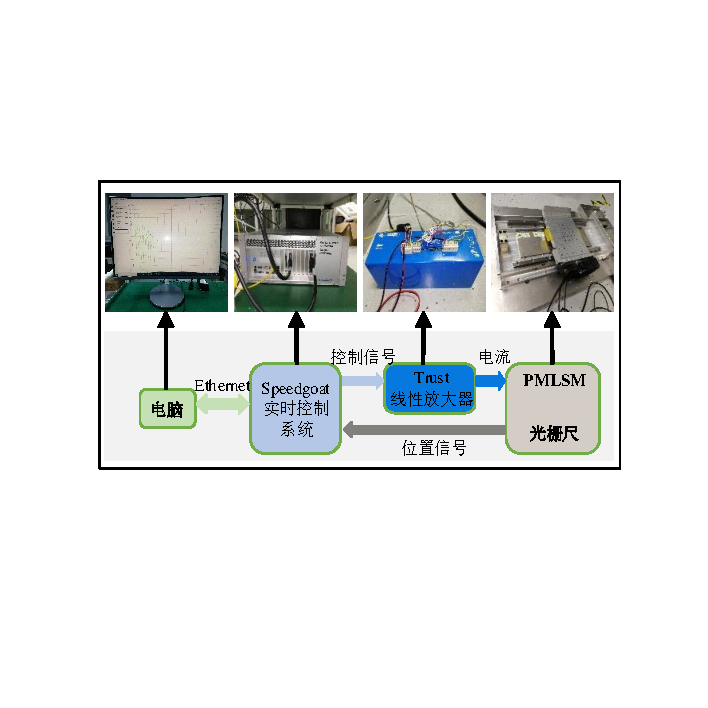
\includegraphics[width=12cm]{figures/实验装置图.pdf}
	\caption{精密直线运动平台实验装置}
	\label{精密直线运动平台实验装置}
\end{figure}
\begin{comment}
\begin{table}[H]
	\caption{ACM1-L100-TL80规格参数.}
	\label{电机参数}
	\centering
	\setlength{\tabcolsep}{5mm}
	\begin{tabular}{ccc}
		\toprule[1.5pt]
		规格参数 &值  &单位 \\
		\midrule
		%\hline
		等效质量&0.12&$\text{Ns$^2$/m}$\\
		力常数&72.9&$\text{N/Arms}$\\
		极距&20.0&$\text{mm}$\\
		电感&18.2&$\text{mH}$\\
		最大总线电压&600&$\text{Vdc}$\\
		持续力&306.3&$\text{N}$\\
		峰值力&1321.8&$\text{N}$\\
		持续电流&4.2&$\text{Arms}$\\
		峰值电流&19.2&$\text{Arms}$\\
		反电动势常数&59.5&$\text{Vpeak/m/s}$\\
		电气时间常数&3.8&$\text{ms}$\\
		\bottomrule[1.5pt]
	\end{tabular}
\end{table}
\end{comment}
\subsection{实验设置}
为了测试所提的控制方法对精密直线运动平台的位置跟踪性能和扰动抑制能力,提供了两种不同的输入信号作为参考轨迹:

1)两组正弦信号,如图\ref{正弦参考轨迹}所示。具体参数为:

(a)频率为0.5$\,\text{Hz}$,幅值为10$\,\text{mm}$;

(b)频率为1$\,\text{Hz}$,幅值为10$\,\text{mm}$。
\begin{figure}[H]
	\centering
%	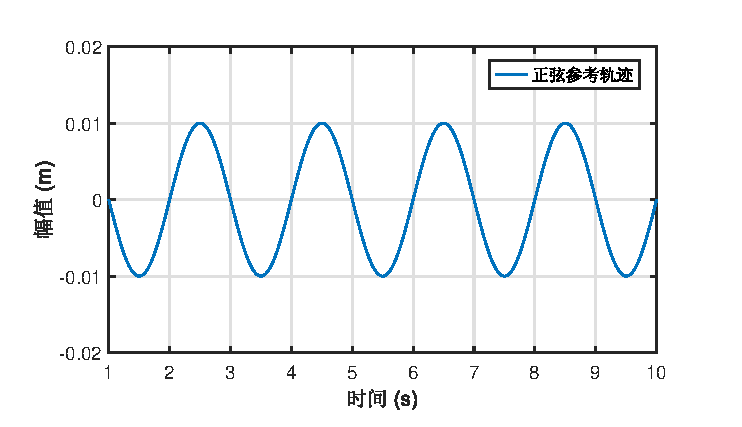
\includegraphics[width=12cm]{figures/正弦参考轨迹.eps}
%	\caption{正弦参考轨迹}
%	\label{正弦参考轨迹}
	\subfloat[0.5\,Hz]
	{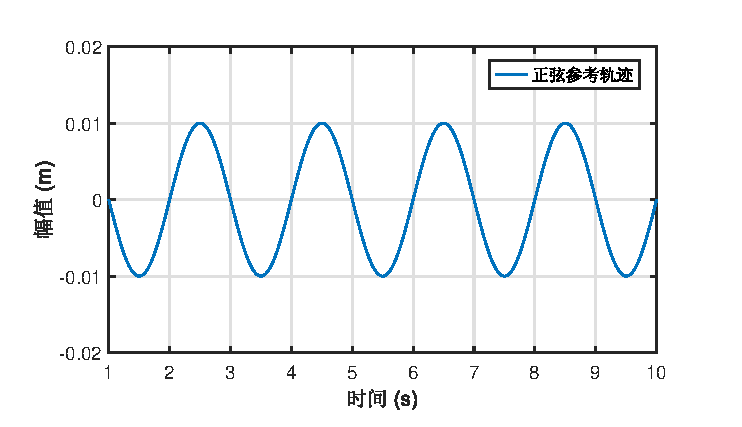
\includegraphics[width=12cm]{figures/正弦参考轨迹.eps}
		\label{Sin1} }\\
	\subfloat[1\,Hz]
	{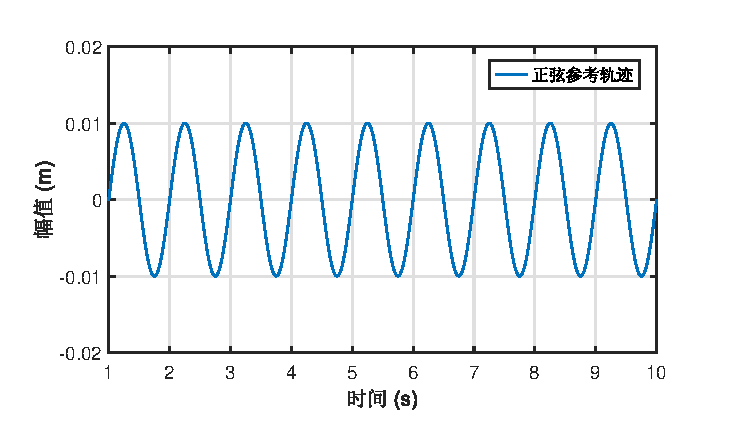
\includegraphics[width=12cm]{figures/正弦参考轨迹1.eps}
		\label{Sin2} }
	\caption{两组不同频率的正弦参考轨迹}
	\label{正弦参考轨迹}
\end{figure}
2)三组三阶轨迹,如图\ref{3组三阶轨迹}所示。具体参数为:

(a) 位移100$\,\text{mm}$,最大速度分别为100$\,\text{mm$/$s}$,最大加速度为4000$\,\text{mm/s$^2$}$;

(b) 位移100$\,\text{mm}$,最大速度分别为150$\,\text{mm$/$s}$,最大加速度为4000$\,\text{mm/s$^2$}$;

(c) 位移100$\,\text{mm}$,最大速度分别为200$\,\text{mm$/$s}$,最大加速度为4000$\,\text{mm/s$^2$}$。

这里为了使得实验结果更加充分,考虑了三种不同的实验设置情况,分别为:

\textbf{实验A.} 无负载情况下对名义模型进行实验测试;

\textbf{实验B.} 有$0.437\,\text{kg}$负载情况下测试对模型参数变化的鲁棒性;

\textbf{实验C.} 在稳态条件下在控制器输出加入$0.5\,\text{V}$持续时间$1\,\text{s}$的外部阶跃扰动(仅正弦输入情况下 5s$\sim$6s)。


\begin{figure}[H]
	\centering
%	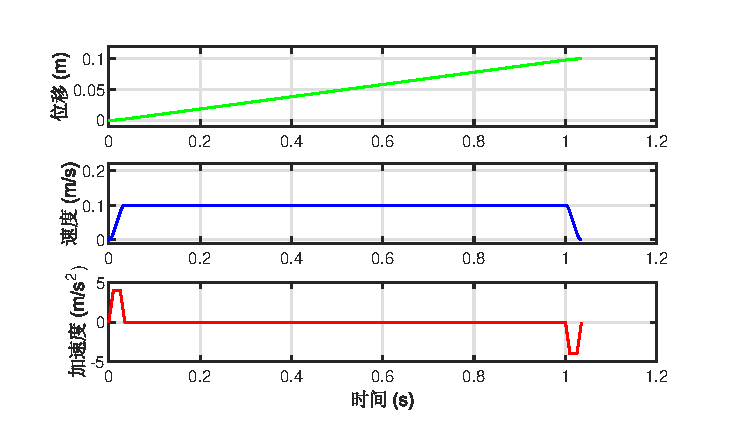
\includegraphics[width=12cm]{figures/三阶轨迹.eps}
%	\caption{三阶S轨迹}\\
    \subfloat[100$\,\text{mm/s}$]
	{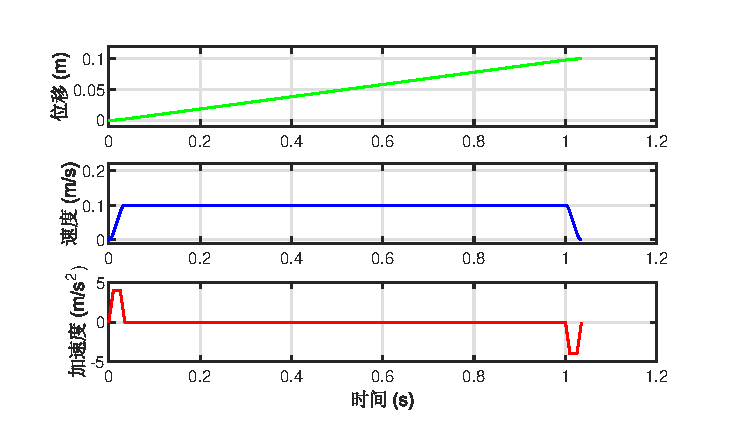
\includegraphics[width=12cm]{figures/三阶轨迹.eps}
		\label{S1} }\\
	\subfloat[150$\,\text{mm/s}$]
	{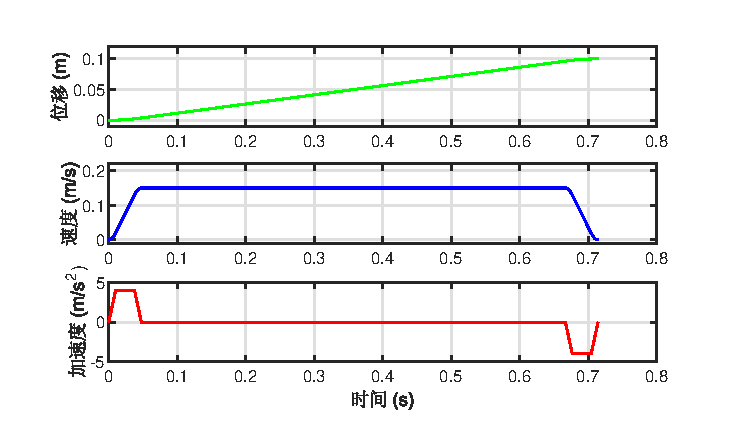
\includegraphics[width=12cm]{figures/三阶轨迹1.eps}
		\label{S2} }\\
	\subfloat[200$\,\text{mm/s}$]
	{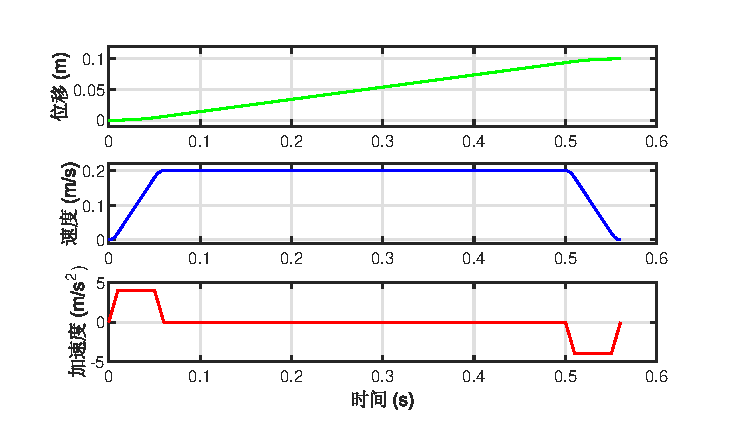
\includegraphics[width=12cm]{figures/三阶轨迹2.eps}
		\label{S3} }
	\caption{不同最大速度的三阶轨迹}
	\label{3组三阶轨迹}
\end{figure}
\section{实验结果与分析}
\subsection{性能评价指标}
为了能够量化地表征控制系统的位置跟踪性能和扰动抑制能力,实验结果的具体性能评价指标设定如下:
\begin{comment}
\begin{enumerate}
	\item 均方根误差(Root Mean Square Error, RMSE):
	\begin{equation}
	\text{RMSE}=\sqrt{\frac{1}{N}\sum_{i=1}^{N}|e(i)|^{2}}
	\end{equation}
	式中,$N$为观测位置跟踪数据的总个数。
	\item 最大绝对误差(Maximum Absolute Error, MAE):
	\begin{equation}
	\text{MAE}=\text{max}\left|e(i)\right|,\,i \in\{1, \ldots, N\}
	\end{equation}
	式中,$N$为观测位置跟踪数据的总个数。
	\item 平均绝对误差(Mean Absolute Deviation, MAD):
	\begin{equation}
	\text{MAD}=\frac{1}{N}\sum_{i=1}^{N}|e(i)|, i \in\{1, \ldots, N\}
	\end{equation}
	式中,$N$为观测位置跟踪数据的总个数。
	\item 移动平均值(Moving Average, MA):
	\begin{equation}
	\text{MA}(i)=\frac{1}{n_e} \sum_{j=i-n_e / 2}^{i+n_e / 2-1} e(j), i \in\{1, \ldots, N\}
	\end{equation}
	移动标准差(Moving Standard Deviation, MSD)\cite{butler2011position}。
	\\
	\begin{equation}
	\text{MSD}(i)=\sqrt{\frac{1}{n_e} \sum_{j=i-n_e / 2}^{i+n_e / 2-1}\left[e(j)-\text{MA}(i)\right]^{2}}, i \in\{1, \ldots, N\}
	\end{equation}
	式中,$n_e\in N^{+}$表示曝光时间窗内的数据个数,其值等于曝光时间除以系统采样时间;$N$为观测位置跟踪数据的总个数。MA和MSD在实际半导体装备中,常用作评价系统位置跟踪性能的指标。以光刻机为例,MA用来表征曝光期间的平均位置误差,代表位置跟踪误差的低频成分;MSD用来表征运动台的定位精度,代表位置跟踪误差的高频成分。因为光刻机系统的关键尺寸和套刻精度都与MA和MSD相关,因此,MA和MSD指标性能至关重要。本文的实验平台虽然不是基于光刻机,但是仍然可以用MA和MSD来作为评价指标对所提方法在精密直线运动平台上跟踪三阶轨迹的位置跟踪性能进行表征\cite{付雪微0有铁芯直线电机推力波动的分析与补偿方法研究}。
	\begin{comment}
	\item 位置误差的方差($S^2$):
	\begin{equation}
	S^{2}=\sum_{i=1}^{N}|e(i)-\bar{e}|^{2}, \forall i \in\{1, \ldots, N\}, \bar{e}=\frac{1}{N} \sum_{i=1}^{N} e(i), \forall i \in\{1, \ldots, N\}
	\end{equation}
	$S^2$表征了所观测的位置跟踪误差的平均波动情况。
\end{enumerate}
\end{comment}

	1. 均方根误差(Root Mean Square Error, RMSE):
	\begin{equation}
	\text{RMSE}=\sqrt{\frac{1}{N}\sum_{i=1}^{N}|e(i)|^{2}}
	\end{equation}
	式中,
	
	$N$为所观测位置跟踪误差数据的总个数。
	
	2. 最大绝对误差(Maximum Absolute Error, MAE):
	\begin{equation}
	\text{MAE}=\text{max}\left|e(i)\right|,\,i \in\{1, \ldots, N\}
	\end{equation}
	式中,
	
	$N$为所观测位置跟踪误差数据的总个数。
	
	3. 平均绝对误差(Mean Absolute Deviation, MAD):
	\begin{equation}
	\text{MAD}=\frac{1}{N}\sum_{i=1}^{N}|e(i)|, i \in\{1, \ldots, N\}
	\end{equation}
	式中,
	
	$N$为所观测位置跟踪误差数据的总个数。
	
	4. 移动平均值(Moving Average, MA),
	\begin{equation}
	\text{MA}(i)=\frac{1}{n_e} \sum_{j=i-n_e / 2}^{i+n_e / 2-1} e(j), i \in\{1, \ldots, N\}
	\end{equation}
	
	移动标准差(Moving Standard Deviation, MSD)\cite{butler2011position}。	(MA和MAS指标仅用于三阶轨迹位置跟踪实验)
	\begin{equation}
	\text{MSD}(i)=\sqrt{\frac{1}{n_e} \sum_{j=i-n_e / 2}^{i+n_e / 2-1}\left[e(j)-\text{MA}(i)\right]^{2}}, i \in\{1, \ldots, N\}
	\end{equation}
	式中,
	
	$n_e\in N^{+}$表示曝光时间窗内的数据个数,其值等于曝光时间除以系统采样时间;
	
	$N$为所观测位置跟踪误差数据的总个数。MA和MSD在实际半导体装备中,常用作评价系统位置跟踪性能的指标。以光刻机为例,MA用来表征曝光期间的平均位置误差,代表位置跟踪误差的低频成分;MSD用来表征运动台的定位精度,代表位置跟踪误差的高频成分。因为光刻机系统的关键尺寸和套刻精度都与MA和MSD相关,因此,MA和MSD指标性能至关重要。本文的实验平台虽然不是基于光刻机,但是仍然可以用MA和MSD来作为评价指标对所提方法在精密直线运动平台上跟踪三阶轨迹的位置跟踪性能
	进行表征\cite{付雪微0有铁芯直线电机推力波动的分析与补偿方法研究}。
\begin{comment}
	\item 位置误差的方差($S^2$):
	\begin{equation}
	S^{2}=\sum_{i=1}^{N}|e(i)-\bar{e}|^{2}, \forall i \in\{1, \ldots, N\}, \bar{e}=\frac{1}{N} \sum_{i=1}^{N} e(i), \forall i \in\{1, \ldots, N\}
	\end{equation}
	$S^2$表征了所观测的位置跟踪误差的平均波动情况。
}
\end{comment}
\subsection{递推最小二乘积分滑模控制器实验结果分析}
基于RLS的积分滑模控制方法的主要优势就是能够实现自适应逆模型前馈控制以及定位力扰动主要成分的自适应前馈补偿,同时积分滑模反馈控制保证了闭环系统的渐近稳定性。这里为了体现逆模型前馈的性能,选择三阶轨迹作为输入参考信号进行实验验证,实验分别在实验A和实验B情况下完成,主要在于对比改进前和改进后二者的瞬态性能和跟踪精度,下面详细介绍实验情况并进行结果分析。

%为了公平地比较本文所提的基于改进型递推最小二乘的积分滑模控制方法(Improved Recursive Least Square Integral Sliding Mode Control, IRLSISMC)

为了公平地比较IRLSISMC与TRLSISMC的性能,将二者共有的参数保持一致,通过调试优化,这里分别将二者的参数设置如下:

1. TRLSISMC:
\begin{equation}
\lambda=800,\,\eta=3,\,\beta=20
\end{equation}



2. IRLSISMC:
\begin{equation}
\lambda=800,\,\eta=3,\,\beta=20,\,\zeta=0.999
\end{equation}
下面具体介绍两种实验情况下,TRLSISMC和IRLSISMC方法的实验情况。

(1)实验A

实验A中,系统名义模型采用事先辨识好的等效质量$M_e=\text{0.12$\,$Vs$^{2}$/m}$,测试TRLSISMC与提出的IRLSISMC在名义模型下的位置跟踪性能,其中,输入的参考轨迹为不同最大速度的三阶轨迹,得到的位置跟踪误差曲线如图\ref{不同最大速度三阶S轨迹名义模型情况下位置跟踪误1}所示。



这种情况下,影响系统位置跟踪性能的主要因素是系统的定位力、摩擦力以及机械系统本身的模态。从位置跟踪误差曲线可以看到,在相同最大速度情况下,两种方法在加减速段的位置跟踪误差没有明显区别,这是因为加减速段主要发挥作用的仍然是逆模型前馈部分。而IRLSISMC方法匀速段的位置跟踪误差明显小于TRLSISMC方法匀速段的位置跟踪误差,这是因为匀速阶段粘滞摩擦力近似为定值,定位力扰动是其扰动的主要来源,而前者在其回归向量中引入了定位力基频成分的扰动形式,能够有效地对定位力扰动进行实时在线补偿。纵向分析不同速度之间,可以发现随着速度的增大,加速段的误差峰值有一定的增加,这主要是因为精密直线运动平台系统的粘滞摩擦与速度相关,高速情况下系统的粘滞摩擦力会更加明显,而且在加速阶段,系统往往需要更大的推力,因此会导致系统高速情况下加速阶段的位置跟踪误差较低速情况时更大一些。
\begin{figure}[H]\centering
	\subfloat[100$\,\text{mm/s}$]
	{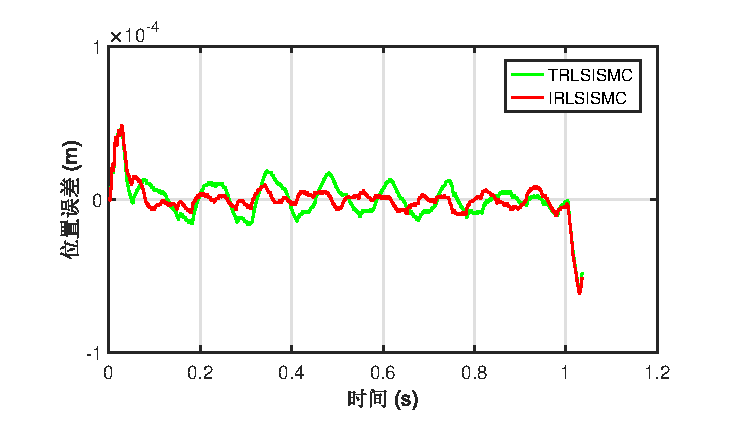
\includegraphics[width=12cm]{figures/rls100E.eps}
		\label{rls100mm} }\\
	\subfloat[150$\,\text{mm/s}$]
	{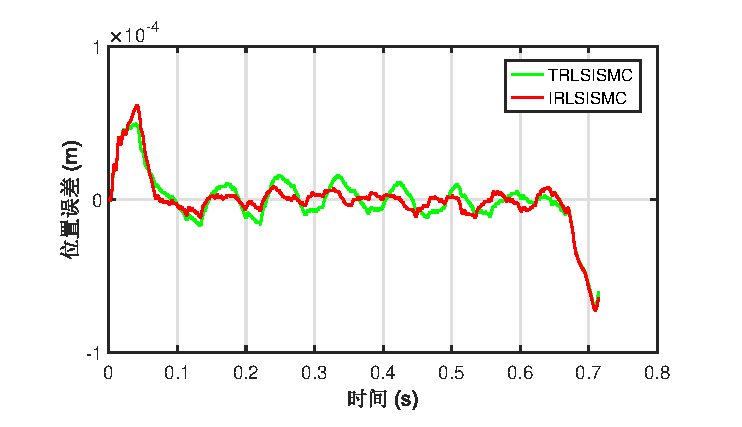
\includegraphics[width=12cm]{figures/rls150E.eps}
		\label{rls150mm} }\\
	\subfloat[200$\,\text{mm/s}$]
	{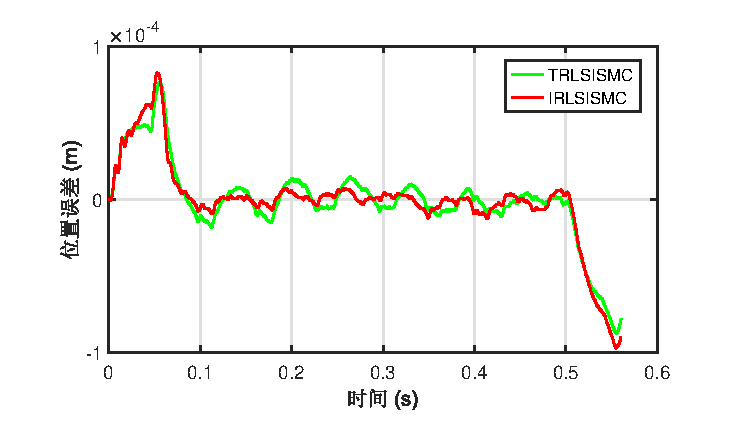
\includegraphics[width=12cm]{figures/rls200E.eps}
		\label{rls200mm} }
	\caption{不同最大速度三阶轨迹名义模型情况下位置跟踪误差}\label{不同最大速度三阶S轨迹名义模型情况下位置跟踪误1}
\end{figure}
为了进一步评价两种控制方法在精密直线运动平台上的控制性能,基于前面提到的性能评价指标对实验A中两种控制方法在匀速阶段的控制性能进行量化表征,具体的性能评价指标RMSE、MAE和MAD的结果如表\ref{实验A1}所示。需要说明的是,由于最大速度不同,因此三种速度情况下,用于计算性能评价指标的数据长度并不一致,具体为:1)100$\,\text{mm/s}$速度情况下,位置跟踪误差如图\ref{rls100mm}所示,选取0.1\,s$\sim$1\,s为所关心的数据段;2)150$\,\text{mm/s}$速度情况下,位置跟踪误差如图\ref{rls150mm}所示,选取0.1\,s$\sim$0.6\,s为所关心的数据段;3)200$\,\text{mm/s}$速度情况下,位置跟踪误差如图\ref{rls200mm}所示,选取0.1\,s$\sim$0.5\,s为所关心的数据段。
\begin{table}[H]
	\caption{实验A中不同最大速度三阶轨迹位置跟踪性能}
	\label{实验A1}
	\centering
	\setlength{\tabcolsep}{3mm} 
	\begin{tabular}{ccccc}
		\toprule[1.5pt]
		& \text{参考轨迹} & RMSE ($\text{$\upmu$m}$) & MAE ($\text{$\upmu$m}$) & $\text{MAD}$($\text{$\upmu$m}$)   \\ 
		\midrule
		\multirow{3}{*}{TRLSISMC}     
		%& C             & 9.57      & 41.4 &0  &0    \\
		& 100\,$\text{mm/s }$        & 8.37      & 18.6 &7.14   \\  
		& 150\,$\text{mm/s }$        & 8.27      & 16.8 &7.24     \\ 
		& 200\,$\text{mm/s }$        & 7.25      & 18.5 &6.06     \\
		\midrule
		\multirow{3}{*}{IRLSISMC} 
		& 100\,$\text{mm/s }$        & 4.28      & 10.8 &3.50  \\  
		& 150\,$\text{mm/s }$        & 4.43      & 11.7 &3.47     \\ 
		& 200\,$\text{mm/s }$        & 4.30      & 12.5 &3.37     \\
		\bottomrule[1.5pt]
	\end{tabular}
\end{table}

分析表格中的结果,可以发现,100\,$\text{mm/s}$三阶轨迹输入情况下,IRLSISMC方法的RMSE可以保持在4\,$\upmu$$\text{m}$附近,而TRLSISMC方法的MAE则在8\,$\upmu$$\text{m}$附近,说明前者的位置跟踪性能更加稳定,即位置跟踪误差的波动较小。IRLSISMC方法的MAE可以保持在11\,$\upmu$$\text{m}$附近,而TRLSISMC方法的MAE则在18\,$\upmu$$\text{m}$附近,说明IRLSISMC方法在匀速段的扰动抑制能力明显优于TRLSISMC方法,同时,MAD的结果也说明了IRLSISMC方法的位置跟踪误差整体较小。综合考虑不同速度下性能指标的变化情况,可以发现,随着速度的增加,两种控制方法的性能指标变化均不大,说明两种方法都比较能够适应速度变化的情况,不过IRLSISMC的位置跟踪精度和扰动抑制能力更好。

(2) 实验B

实验B中,在实验A的基础上添加了$0.437\,\text{kg}$负载,测试TRLSISMC与提出的IRLSISMC对系统模型参数变化的鲁棒性,得到的位置跟踪误差曲线如图\ref{不同最大速度三阶S轨迹有负载情况下位置跟踪误2}所示。定性分析,可以发现,当系统模型参数发生变化时,两种控制方法的位置跟踪性能仍然能够保持相对稳定的情况,与实验A中相比,可以清晰地看出,实验B中的位置跟踪误差曲线几乎维持在同一水平。

\begin{figure}[H]\centering
	\subfloat[100$\,\text{mm/s}$]
	{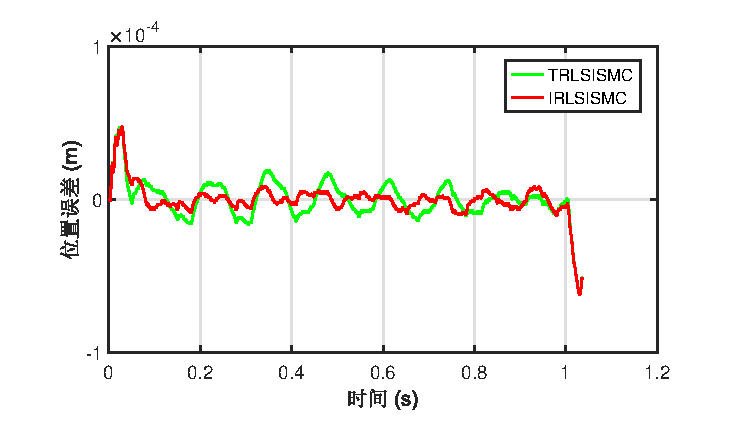
\includegraphics[width=12cm]{figures/rls100LoadE.eps}
		\label{rls100mmLoad} }\\
	\subfloat[150$\,\text{mm/s}$]
	{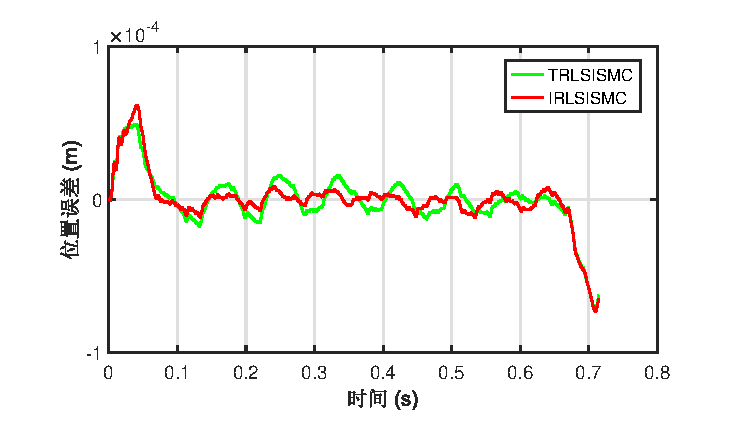
\includegraphics[width=12cm]{figures/rls150LoadE.eps}
		\label{rls150mmLoad} }\\
	\subfloat[200$\,\text{mm/s}$]
	{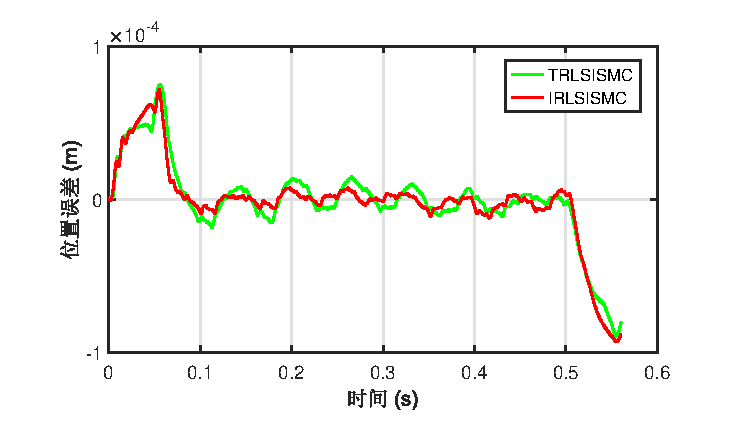
\includegraphics[width=12cm]{figures/rls200LoadE.eps}
		\label{rls200mmLoad} }
	\caption{不同最大速度三阶轨迹有负载情况下位置跟踪误差}\label{不同最大速度三阶S轨迹有负载情况下位置跟踪误2}
\end{figure}

为了更加清楚地认识两种控制方法对于系统模型参数变化的鲁棒性,还需要基于前面提到的性能指标对其位置跟踪误差曲线进行定量分析,
具体的性能评价指标与实验A中一致,结果如表\ref{实验B2}所示。
\begin{table}[H]
	\caption{实验B中不同最大速度三阶轨迹位置跟踪性能.}
	\label{实验B2}
	\centering
	\setlength{\tabcolsep}{3mm} 
	\begin{tabular}{ccccc}
		\toprule[1.5pt]
		& \text{参考轨迹} & RMSE ($\text{$\upmu$m}$) & MAE ($\text{$\upmu$m}$) & $\text{MAD}$($\text{$\upmu$m}$)   \\ 
		\midrule
		\multirow{3}{*}{TRLSISMC}     
		%& C             & 9.57      & 41.4 &0  &0    \\
		& 100\,$\text{mm/s }$        & 8.41      & 18.7 &7.15   \\  
		& 150\,$\text{mm/s }$        & 8.30      & 17.8 &7.25     \\ 
		& 200\,$\text{mm/s }$        & 7.27      & 18.5 &6.06     \\
		\midrule
		\multirow{3}{*}{IRLSISMC} 
		& 100\,$\text{mm/s }$       & 4.26      & 10.8 &3.50  \\  
		& 150\,$\text{mm/s }$       & 4.37      & 11.7 &3.45     \\ 
		& 200\,$\text{mm/s }$       & 4.32      & 12.2 &3.43     \\
		\bottomrule[1.5pt]
	\end{tabular}
\end{table}



分析表格中的结果,容易发现,与实验A对比,实验B中的性能指标与实验A中的性能指标相差并不大,这充分说明了两种方法均能够很好地应对系统模型参数的摄动,但IRLSISMC方法的位置跟踪性能仍然优于TRLSISMC。

对实验A和实验B中的三阶轨迹匀速段位置跟踪误差进行了MA和MSD分析,结果如图\ref{不同速度情况下位置跟踪误差MA、MSD曲线2}所示。可以清楚地看到,当运行速度提高时,TRLSISMC方法的MA和MSD均有不同程度的增大,而IRLSISMC方法的MA和MSD都是稳定地维持在较低水平,这充分说明了IRLSISMC方法的位置跟踪性能优于TRLSISMC方法,位置跟踪精度以及位置跟踪误差的稳定性都有很大的提升。

从具体的数值角度来分析,在最大速度为100\,$\text{mm/s}$且无负载情况时,TRLSISMC方法匀速段跟踪误差的MA最大为8.93\,$\text{$\upmu$m}$,MSD最大为13.4\,$\text{$\upmu$m}$,而所提的IRLSISMC方法匀速段跟踪误差的MA最大为3.99\,$\text{$\upmu$m}$,MSD最大为6.27\,$\text{$\upmu$m}$,与TRLSISMC方法相比,IRLSISMC方法的位置跟踪性能得到了极大的提升。在有负载的情况下,MA和MSD的值也几乎保持一致,IRLSISMC方法的MA和MSD分别为4.00\,$\text{$\upmu$m}$和6.23\,$\text{$\upmu$m}$,这一结果从位置跟踪误差的整体性能层面也验证了所提IRLSISMC方法能够有效地提高系统位置跟踪精度,并对系统模型参数变化有一定的鲁棒性。

在最大速度为200\,$\text{mm/s}$且无负载情况时,TRLSISMC方法匀速段跟踪误差的MA最大为8.11\,$\text{$\upmu$m}$,MSD最大为10.7\,$\text{$\upmu$m}$,而所提的IRLSISMC方法匀速段跟踪误差的MA最大为6.31\,$\text{$\upmu$m}$,MSD最大为5.13\,$\text{$\upmu$m}$。纵向对比不同速度情况下匀速段跟踪误差的MA和MSD的变化,可以发现系统运行速度从100\,$\text{mm/s}$到200\,$\text{mm/s}$时,系统的MA和MSD并不是都随着速度的提高而增大的,这主要是因为实验所用精密直线运动平台的摩擦力中包含的Stribeck效应导致系统在高速运行情况下,如第二章公式(\ref{2.11})表示的摩擦力模型所示,摩擦力的非线性特性会相对降低,但是粘滞摩擦力的值仍然是较低速情况下更大一些,这才导致了高速情况下系统的MA会有所增加,而MSD反而会有一定程度的降低,说明这时位置跟踪误差虽然值有所增加,但是却更加均匀,离散程度更小。

\begin{figure}[H]
	\centering
	\subfloat[100$\,\text{mm/s}$三阶S轨迹无负载]{\label{rlsMAMSD100mm无负载}%%
		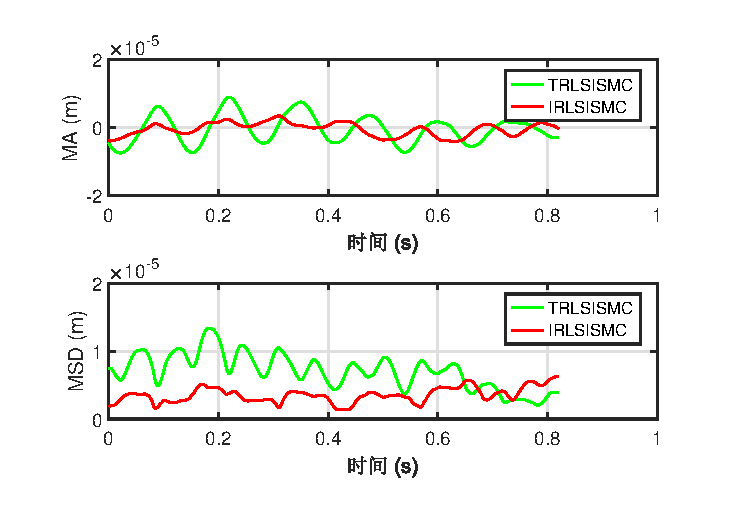
\includegraphics[width=7.6cm]{figures/rlsMAMSD100mm无负载.eps}} 	
	\subfloat[100$\,\text{mm/s}$三阶S轨迹有负载]{\label{rlsMAMSD100mm有负载}%%
		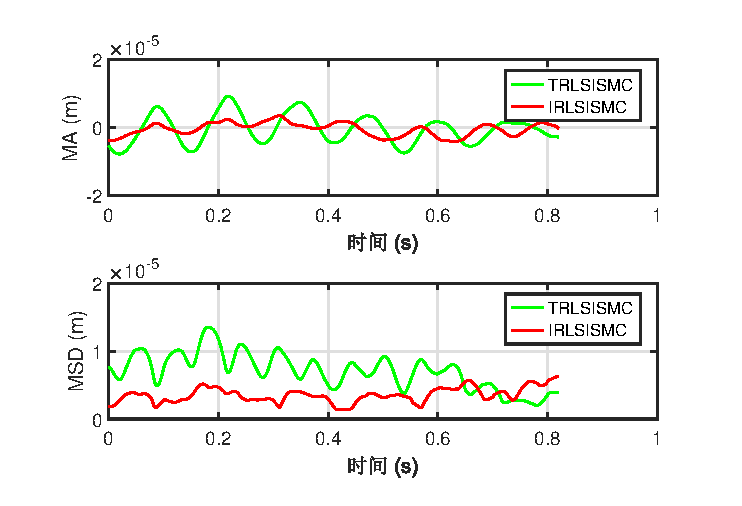
\includegraphics[width=7.6cm]{figures/rlsMAMSD100mm有负载.eps}} \\
	\subfloat[150$\,\text{mm/s}$三阶S轨迹无负载]{\label{rlsMAMSD150mm无负载}%%
		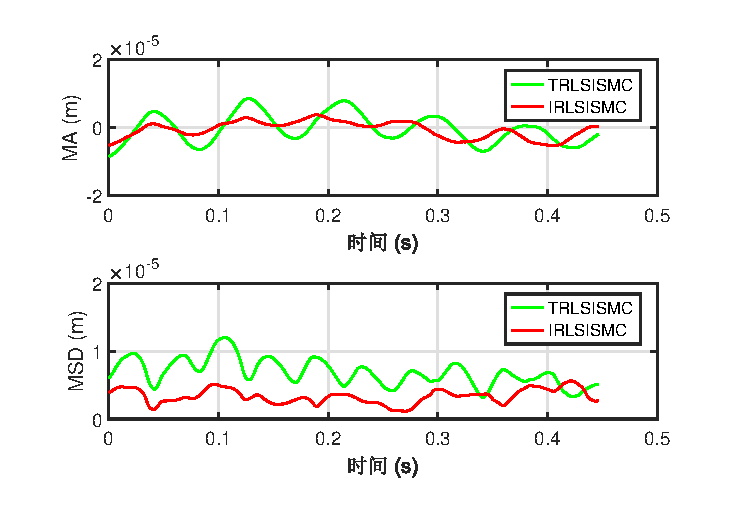
\includegraphics[width=7.6cm]{figures/rlsMAMSD150mm无负载.eps}} 	
	\subfloat[150$\,\text{mm/s}$三阶S轨迹有负载]{\label{rlsMAMSD150mm有负载}%%
		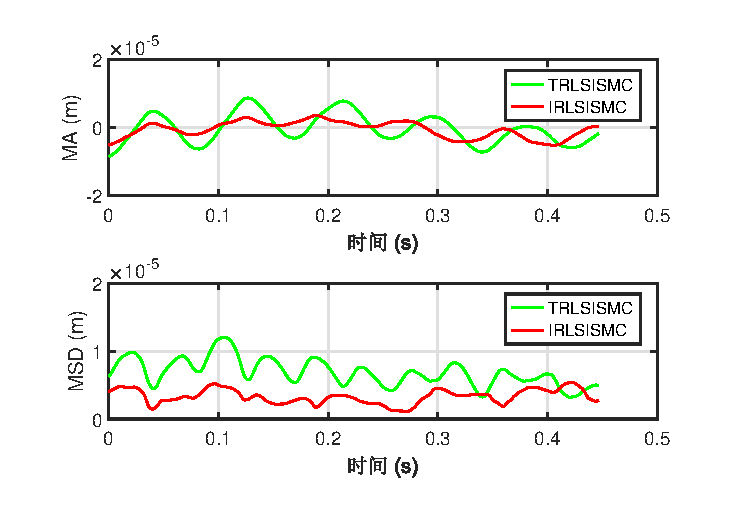
\includegraphics[width=7.6cm]{figures/rlsMAMSD150mm有负载.eps}} \\
	\subfloat[200$\,\text{mm/s}$三阶S轨迹无负载]{\label{rlsMAMSD200mm无负载}%%
		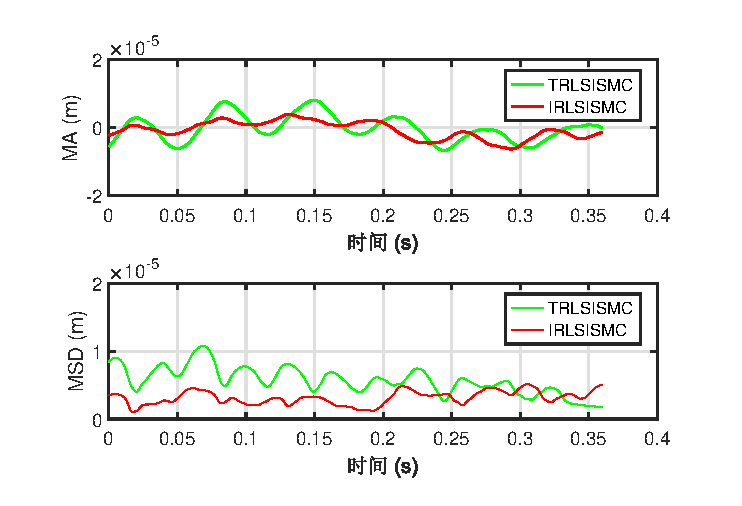
\includegraphics[width=7.6cm]{figures/rlsMAMSD200mm无负载.eps}} 	
	\subfloat[200$\,\text{mm/s}$三阶S轨迹有负载]{\label{rlsMAMSD200mm有负载}%%
		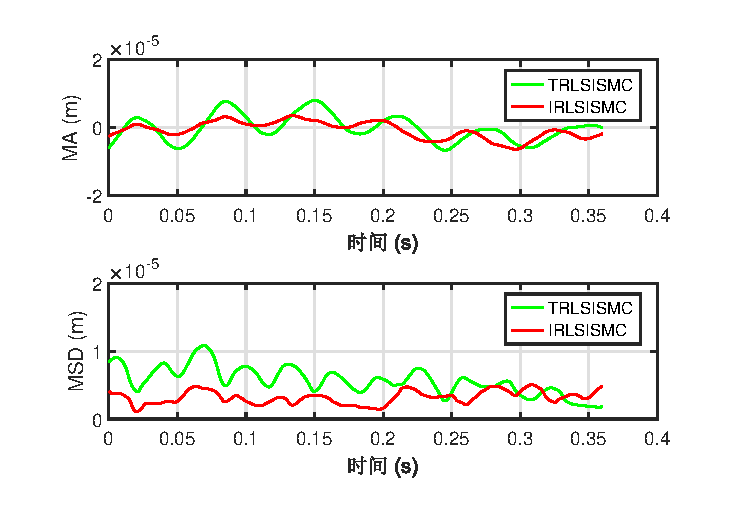
\includegraphics[width=7.6cm]{figures/rlsMAMSD200mm有负载.eps}} \\
	\caption{不同速度情况下位置跟踪误差MA、MSD曲线}
	\label{不同速度情况下位置跟踪误差MA、MSD曲线2}
\end{figure}





\subsection{多核神经网络动态边界层滑模控制器实验结果分析}
多核神经网络动态边界层滑模控制方法的提出主要是为了提高精密直线运动平台的位置跟踪性能和扰动抑制能力,这里为了更有力地表明所提方法的有效性以及设计参数对于整个控制系统性能的影响,在两种参考轨迹的输入情况下分别就三种实验情况都与传统RBF神经网络滑模控制进行了对比实验,下面详细介绍实验情况并进行结果分析。

为了公平地比较所提出的多核神经网络动态边界层滑模控制方法(Multi-Kernel Neural Network Sliding Mode Control, MNNSMC)与传统RBF神经网络自适应滑模控制方法(Adaptive Sliding Mode Control, ASMC),将二者共同的参数设置一致,只保留所提出的方法的特有的参数设置可调。通过调试优化,这里分别将二者的参数设置如下:
\begin{enumerate}
	\item 传统ASMC:
	\begin{equation}
	\lambda =800\text{,}\,\eta =3\text{,}\,\gamma =2\cdot\text{exp}(-4)\text{,}\,\Delta =0.005
	\end{equation}
	\item MNNSMC:
	\begin{equation}
	\begin{aligned}
	&\lambda=800\text{,}\,\eta =3\text{,}\,{{\Delta}_{0}}=0.005\text{,}\,\alpha=3\text{,} \\ 
	&\textbf{ }\!\!{\gamma}=\text{diag}([\underbrace{2\text{,}\cdots\text{,}\,2}_{N_h}\text{,}\underbrace{1\text{,}\cdots\text{,}\,1}_{2N_t}\text{,}\,0.5]\cdot\exp(-4)) \\ 
	\end{aligned}
	\end{equation}
	式中, $N_h$\,=\,$5$,即高斯核函数的节点有5个;$N_t$\,=\,$4$,即三角核函数的节点有4对,分别对应4个定位力主要频率;Sigmoid核函数的节点只有1个。
\end{enumerate}

三种实验设置下,对本文所提出的MNNSMC方法与传统ASMC方法在精密直线运动平台上的控制性能进行了验证,下面介绍具体的实验情况。

(1) 实验A

实验A中,系统名义模型仍采用事先辨识好的等效质量$M_e=\text{0.12$\,$Vs$^{2}$/m}$,测试传统ASMC与提出的MNNSMC在名义模型下的位置跟踪性能,不同频率的正弦参考轨迹与不同最大速度的三阶轨迹作为位置参考输入信号,得到的位置跟踪误差曲线如图\ref{不同频率正弦参考轨迹名义模型情况下位置跟踪误差}和图\ref{不同最大速度三阶S轨迹名义模型情况下位置跟踪误}所示。
如前面提到的,实验A的设置下,影响系统位置跟踪性能的主要因素是系统的定位力、摩擦力以及机械系统本身的模态。

当输入正弦变化的位置参考轨迹时,得到的位置跟踪误差曲线如图\ref{不同频率正弦参考轨迹名义模型情况下位置跟踪误差}所示,可以发现,本文提出的MNNSMC方法的位置跟踪误差明显小于ASMC方法,而且对比两种不同频率的正弦信号时能够发现,正弦信号的频率越高,即参考轨迹的速度、加速度越大时,MNNSMC方法的优势体现的越明显,这是因为MNNSMC方法中引入了精密直线运动平台的定位力和摩擦力模型,这种多核神经网络模型能够更有效地适应高速高精度运行要求。可以看到,在正弦频率较高的时,MNNSMC方法的暂态和ASMC相当,但是稳态性能远远优于ASMC方法,这是因为神经网络权重的调节都需要一定的时间,这在实际工程应用对于整定时间要求不太严苛时,是完全可以接受的。


\begin{figure}[H]\centering
	\subfloat[0.5$\,\text{Hz}$]
	{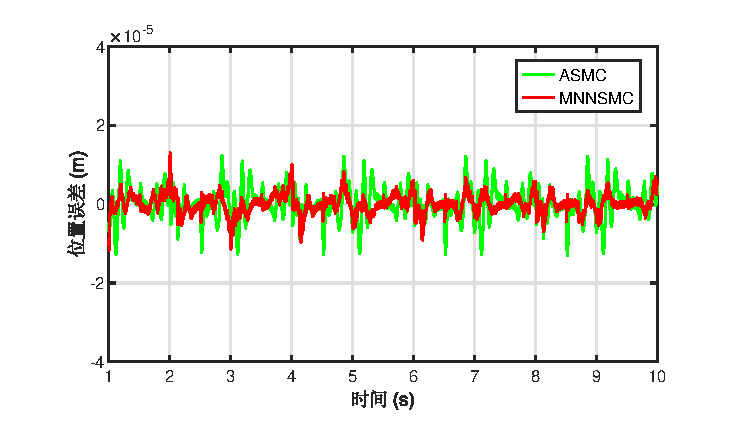
\includegraphics[width=12cm]{figures/正弦05Hz无负载.eps}
		\label{正弦05无负载} }\\
	\subfloat[1$\,\text{Hz}$]
	{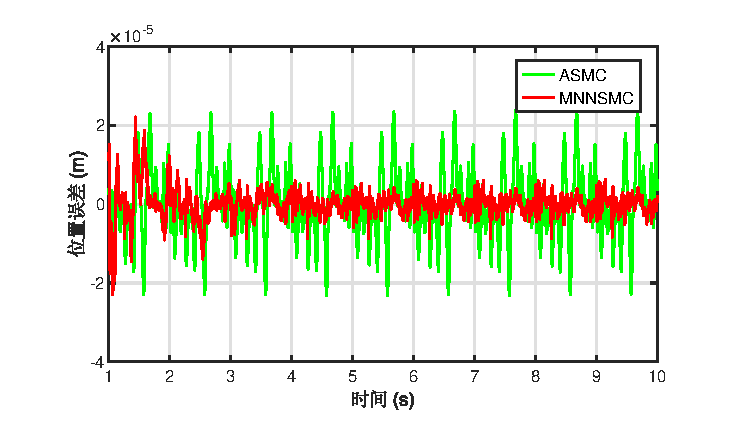
\includegraphics[width=12cm]{figures/正弦1Hz无负载.eps}
		\label{正弦1Hz无负载} }
	\caption{不同频率正弦参考轨迹名义模型情况下位置跟踪误差}\label{不同频率正弦参考轨迹名义模型情况下位置跟踪误差}
\end{figure}
当系统输入不同最大速度的三阶轨迹时,系统位置跟踪误差如图\ref{不同最大速度三阶S轨迹名义模型情况下位置跟踪误}所示,可以发现,本文提出的MNNSMC方法较传统的ASMC方法在加减速段和匀速段的位置跟踪性能方面都有明显的提升。而且随着速度的增加,MNNSMC方法比ASMC方法能够更好地适应高速的情况。仔细对比不同速度情况下的位置跟踪误差曲线,不难发现,MNNSMC方法在加速阶段的位置跟踪误差曲线的峰值有一定的增加,但是仍远小于传统ASMC方法。在匀速阶段,传统ASMC的误差随着速度的增加而增加的较为明显,提出的MNNSMC方法的位置跟踪误差则有减小的趋势,这是因为MNNSMC中提出的动态边界层与速度相关,能够较好地适应高速的情况,而神经网络补偿部分则能够更好地抑制系统内部和外部的总扰动,从而能够提高高速运行情况下的位置跟踪精度和扰动抑制能力。
\\
\begin{figure}[H]\centering
	\subfloat[100$\,\text{mm$/$s}$]
	{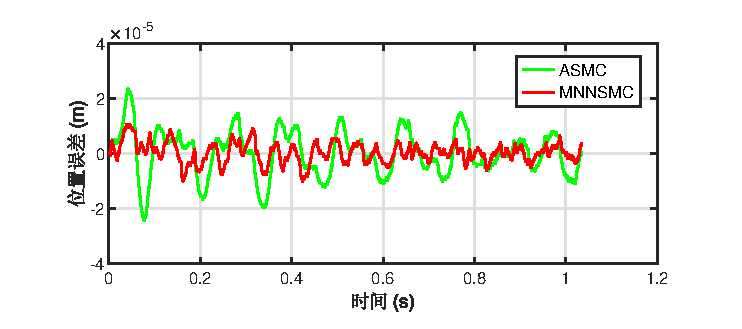
\includegraphics[width=12cm]{figures/S轨迹100无负载.eps}
		\label{S轨迹100无负载} }\\
	\subfloat[150$\,\text{mm$/$s}$]
	{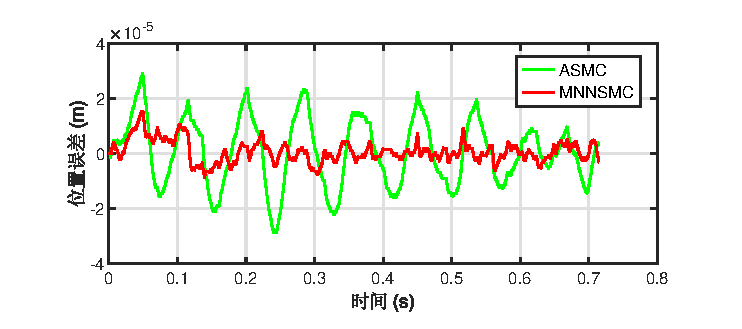
\includegraphics[width=12cm,height=5cm]{figures/S轨迹150无负载.eps}
		\label{S轨迹150无负载} }\\
	\subfloat[200$\,\text{mm$/$s}$]
	{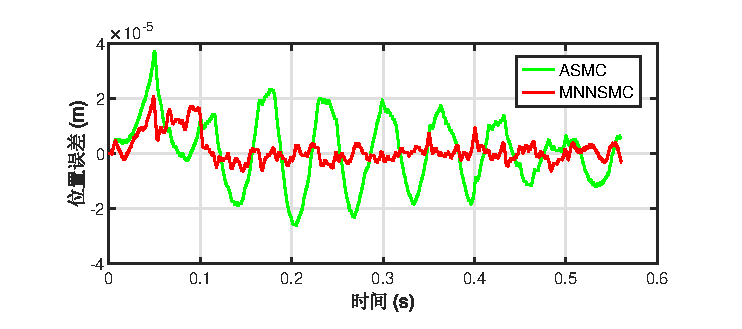
\includegraphics[width=12cm]{figures/S轨迹200无负载.eps}
		\label{S轨迹200无负载} }
	\caption{不同最大速度三阶轨迹名义模型情况下位置跟踪误}\label{不同最大速度三阶S轨迹名义模型情况下位置跟踪误}
\end{figure}

\begin{comment}
\begin{figure}[H]
	\centering
	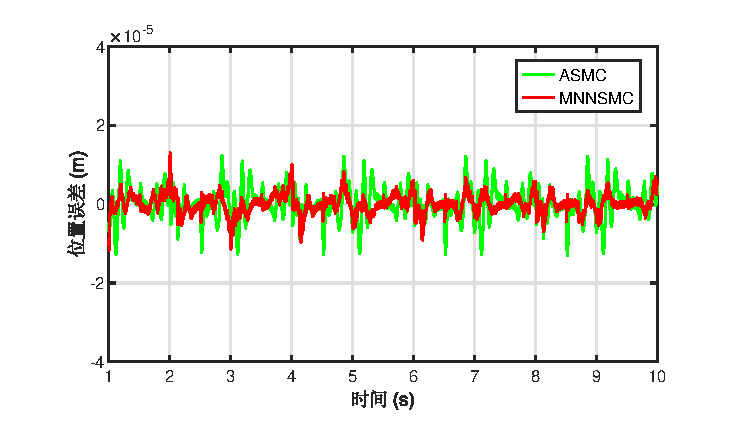
\includegraphics[width=12cm]{figures/正弦05Hz无负载.eps}
	\caption{0.5$\,\text{Hz}$正弦参考轨迹名义模型情况下位置跟踪误差}
	\label{正弦05无负载}
\end{figure}
\begin{figure}[H]
	\centering
	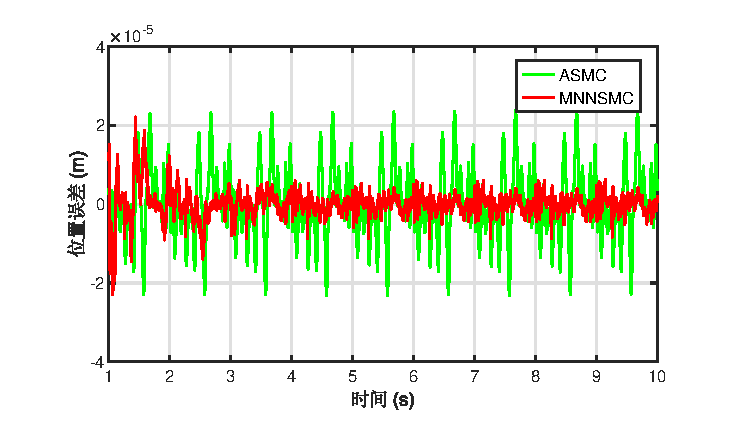
\includegraphics[width=12cm]{figures/正弦1Hz无负载.eps}
	\caption{1$\,\text{Hz}$正弦参考轨迹名义模型情况下位置跟踪误差}
	\label{正弦1Hz无负载}
\end{figure}
\end{comment}



\begin{comment}
\begin{figure}[H]
	\centering
	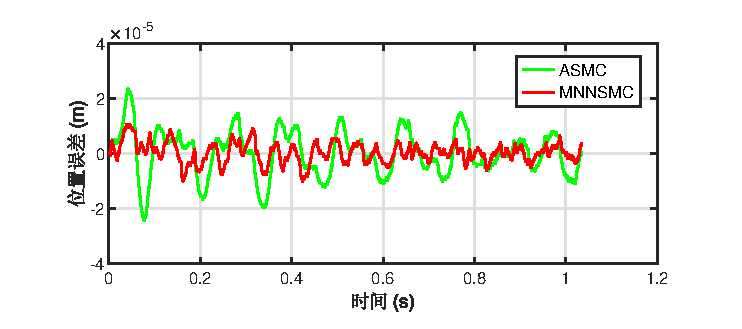
\includegraphics[width=12cm]{figures/S轨迹100无负载.eps}
	\caption{最大速度为100$\,\text{mm$/$s}$的三阶S轨迹名义模型情况下位置跟踪误差}
	\label{S轨迹100无负载}
\end{figure}
\begin{figure}[H]
	\centering
	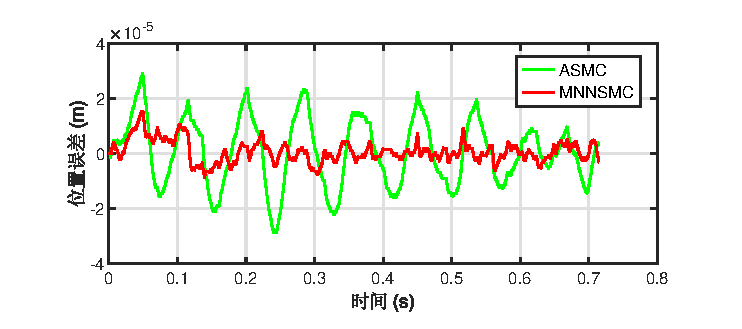
\includegraphics[width=12cm]{figures/S轨迹150无负载.eps}
	\caption{最大速度为150$\,\text{mm$/$s}$的三阶S轨迹名义模型情况下位置跟踪误差}
	\label{S轨迹150无负载}
\end{figure}
\begin{figure}[H]
	\centering
	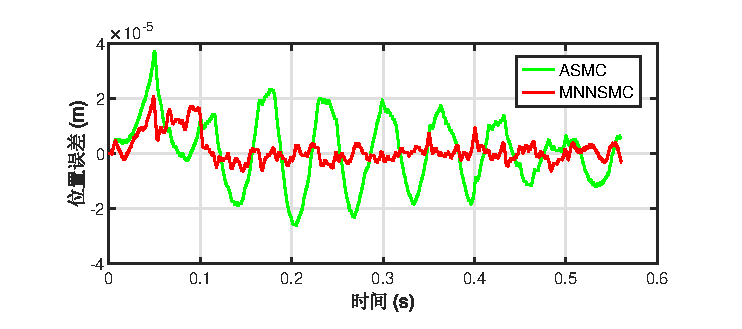
\includegraphics[width=12cm]{figures/S轨迹200无负载.eps}
	\caption{最大速度为200$\,\text{mm$/$s}$的三阶S轨迹名义模型情况下位置跟踪误差}
	\label{S轨迹200无负载}
\end{figure}
\end{comment}


为了进一步评价两种基于神经网络的控制方法在精密直线运动平台上的控制性能,这里对实验A中两种控制方法在匀速阶段的控制性能进行量化表征,具体的性能评价指标RMSE、MAE和MAD的结果如表\ref{实验A}所示。需要说明的是,当系统输入三阶轨迹时,由于最大速度不同,用于计算性能评价指标的数据长度并不一致,具体为:1)100$\,\text{mm/s}$速度情况下,位置跟踪误差如图\ref{S轨迹100无负载}所示,选取0.2\,s$\sim$1\,s为所关心的数据段;2)150$\,\text{mm/s}$速度情况下,位置跟踪误差如图\ref{S轨迹150无负载}所示,选取0.2\,s$\sim$0.6\,s为所关心的数据段;3)200$\,\text{mm/s}$速度情况下,位置跟踪误差如图\ref{S轨迹200无负载}所示,选取0.2\,s$\sim$0.5\,s为所关心的数据段。
\begin{table}[H]
	\caption{实验A中不同参考轨迹位置跟踪性能.}
	\label{实验A}
	\centering
	\setlength{\tabcolsep}{3mm} 
	\begin{tabular}{ccccc}
		\toprule[1.5pt]
		& \text{参考轨迹} & RMSE ($\text{$\upmu$m}$) & MAE ($\text{$\upmu$m}$) & $\text{MAD}$($\text{$\upmu$m}$)   \\ 
		\midrule
		\multirow{5}{*}{ASMC}     
		& 0.5Hz         & 4.08      & 13.1 &2.97     \\ 
		& 1Hz           & 8.94      & 23.6 &6.70     \\ 
		%& C             & 9.57      & 41.4 &0  &0    \\
		& 100\,$\text{mm/s }$            & 7.55      & 19.5 &6.13   \\  
		& 150\,$\text{mm/s }$             & 13.1      & 28.6 &11.3     \\ 
		& 200\,$\text{mm/s }$             & 12.2      & 26.0 &10.4     \\
		\midrule
		\multirow{5}{*}{MNNSMC} 
		& 0.5Hz           & 2.37      & 13.1 &1.73    \\ 
		& 1Hz             & 3.47      & 23.0 &2.19     \\ 
		& 100\,$\text{mm/s }$            & 3.31      & 10.1 &2.63  \\  
		& 150\,$\text{mm/s }$             & 2.73      & 9.23 &2.10     \\ 
		& 200\,$\text{mm/s }$             & 2.38      & 9.40 &1.87    \\
		\bottomrule[1.5pt]
	\end{tabular}
\end{table}

分析表格中的结果,可以发现,正弦信号输入情况下,频率为0.5\,Hz时,ASMC与MNNSMC的MAE都为13.1\,$\upmu$$\text{m}$,RMSE和MAD也都相差不大,但是当频率为1Hz时,虽然两种方法MAE的值仍然相差不大,但是MNNSMC方法的RMSE和MAD都小于ASMC方法的一半。这主要是因为当正弦信号频率变高,即参考轨迹的速度变快,扰动带来的影响也会更加明显,主要是粘滞摩擦力近似与速度成正比,而基于传统RBF的ASMC扰动补偿的能力有限,所提出的MNNSMC方法因为在核函数的设计中考虑了摩擦力的模型,因此MNN神经网络的收敛速度会更快,扰动补偿能力也会因此而显著提高。

最大速度为100\,$\text{mm/s}$的三阶轨迹输入情况下,MNNSMC方法的MAE可以保持在10\,$\upmu$$\text{m}$附近,而ASMC方法的MAE则在20\,$\upmu$$\text{m}$附近。前者的RMSE和MAD的值远远低于后者,这充分表明了本文所提MNNSMC方法在提高精密直线运动平台位置跟踪性能方面优于传统ASMC方法。此外,纵向对比不同速度情况下的位置跟踪性能,可以发现,随着速度的增加,ASMC位置跟踪性能的三项评价指标均有一定的恶化,但是MNNSMC方法的各项性能指标则相对较为稳定,这进一步表明MNNSMC的控制性能更优。

(2) 实验B

实验B中,在实验A的基础上添加了$0.437\,\text{kg}$负载,测试传统ASMC与提出的MNNSMC对系统模型参数变化的鲁棒性,得到的位置跟踪误差曲线如图\ref{不同频率正弦参考轨迹有负载情况下位置跟踪误差}和图\ref{不同最大速度三阶S轨迹有负载情况下位置跟踪误}所示。

当不同频率的正弦参考轨迹输入时,得到的系统位置跟踪误差曲线如图\ref{不同频率正弦参考轨迹有负载情况下位置跟踪误差}所示,与实验A相比,可以直观地看到,实验B的位置跟踪误差曲线没有明显的变化,这充分说明了两种基于神经网络的控制方法对于均能够很好地应对系统模型参数摄动,即鲁棒性好。

\begin{figure}[H]\centering
	\subfloat[0.5$\,\text{Hz}$]
	{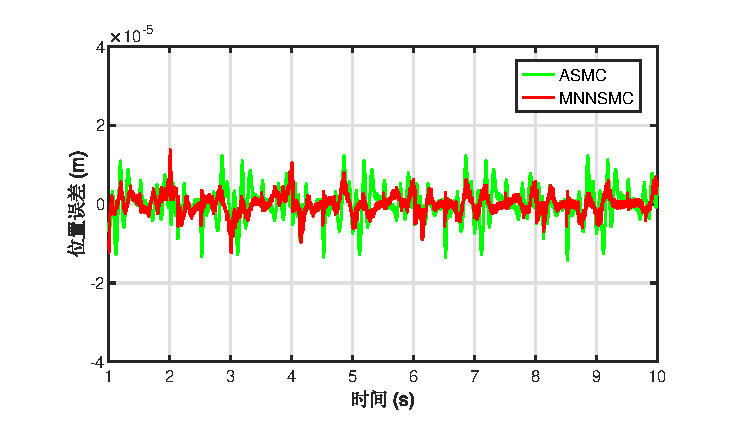
\includegraphics[width=12cm]{figures/正弦05Hz有负载.eps}
		\label{正弦05有负载} }\\
	\subfloat[1$\,\text{Hz}$]
	{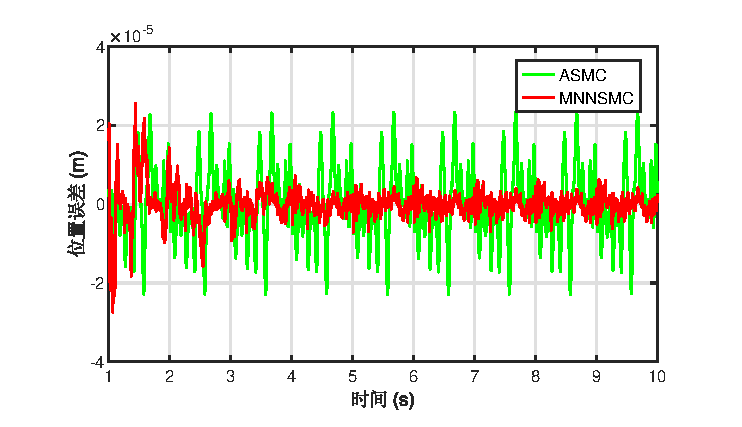
\includegraphics[width=12cm]{figures/正弦1Hz有负载.eps}
		\label{正弦1Hz有负载} }
	\caption{不同频率正弦参考轨迹有负载情况下位置跟踪误差}\label{不同频率正弦参考轨迹有负载情况下位置跟踪误差}
\end{figure}
当不同最大速度的三阶轨迹输入时,得到的系统位置跟踪误差曲线如图\ref{不同最大速度三阶S轨迹有负载情况下位置跟踪误}所示,仔细观察可以发现,与实验A相比,实验B中传统ASMC方法在加速阶段的位置跟踪误差峰值有略微的增加,这是因为加速阶段需要的推力有略微的增加,而本文提出的MNNSMC方法在加速阶段的位置跟踪误差则没有明显的变化。此外,在匀速阶段,两种方法的位置跟踪误差曲线均无明显变化,这同样说明了所提方法对于系统模型参数摄动具有较好的鲁棒性。


\begin{figure}[H]\centering
	\subfloat[100$\,\text{mm$/$s}$]
	{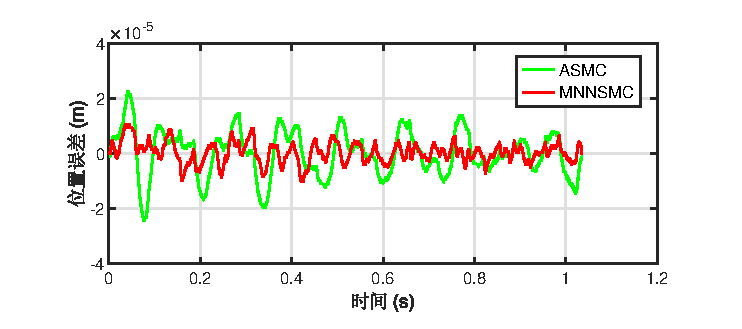
\includegraphics[width=12cm]{figures/S轨迹100有负载.eps}
		\label{S轨迹100有负载} }\\
	\subfloat[150$\,\text{mm$/$s}$]
	{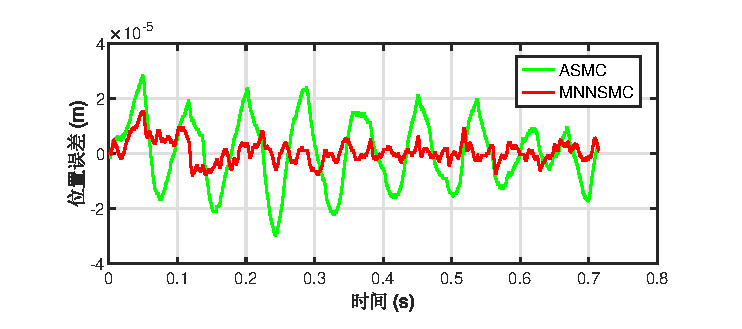
\includegraphics[width=12cm]{figures/S轨迹150有负载.eps}
		\label{S轨迹150有负载} }\\
	\subfloat[200$\,\text{mm$/$s}$]
	{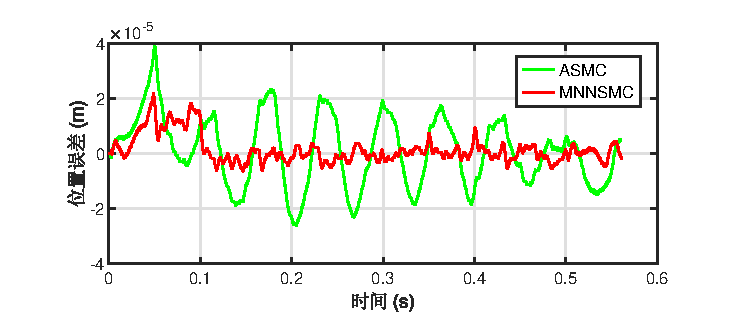
\includegraphics[width=12cm]{figures/S轨迹200有负载.eps}
		\label{S轨迹200有负载} }
	\caption{不同最大速度三阶轨迹有负载情况下位置跟踪误}\label{不同最大速度三阶S轨迹有负载情况下位置跟踪误}
\end{figure}
为了更具体地表征实验B中精密直线运动平台的位置跟踪性能,将定量分析的性能指标数据总结在表\ref{不同最大速度三阶S轨迹有负载情况下位置跟踪误}中,关心的数据段与实验A中一致:1)100$\,\text{mm/s}$速度情况下,位置跟踪误差如图\ref{S轨迹100无负载}所示,选取0.2\,s$\sim$1\,s为所关心的数据段;2)150$\,\text{mm/s}$速度情况下,位置跟踪误差如图\ref{S轨迹150无负载}所示,选取0.2\,s$\sim$0.6\,s为所关心的数据段;3)200$\,\text{mm/s}$速度情况下,位置跟踪误差如图\ref{S轨迹200无负载}所示,选取0.2\,s$\sim$0.5\,s为所关心的数据段。
\begin{comment}
\begin{figure}[H]
	\centering
	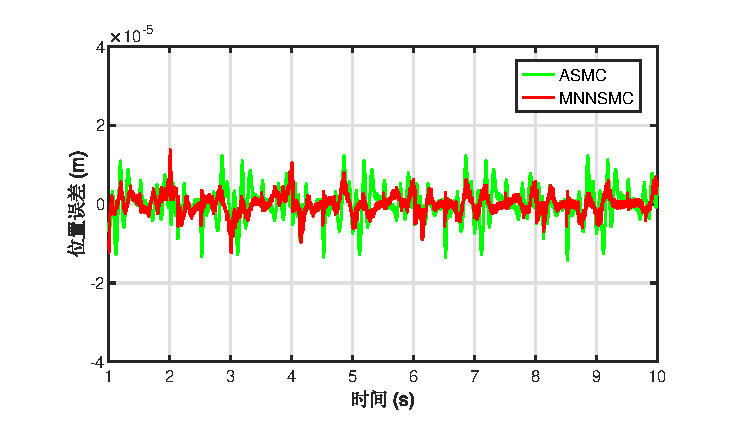
\includegraphics[width=12cm]{figures/正弦05Hz有负载.eps}
	\caption{0.5$\,\text{Hz}$正弦参考轨迹有负载情况下位置跟踪误差}
	\label{正弦05有负载}
\end{figure}
\begin{figure}[H]
	\centering
	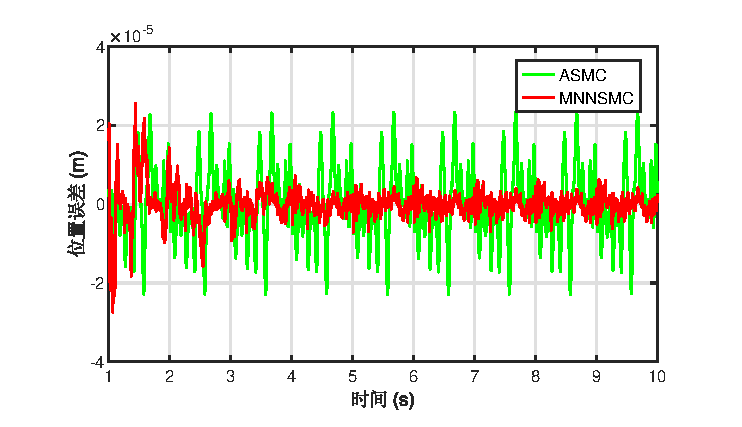
\includegraphics[width=12cm]{figures/正弦1Hz有负载.eps}
	\caption{1$\,\text{Hz}$正弦参考轨迹有负载情况下位置跟踪误差}
	\label{正弦1Hz有负载}
\end{figure}
\begin{figure}[H]
	\centering
	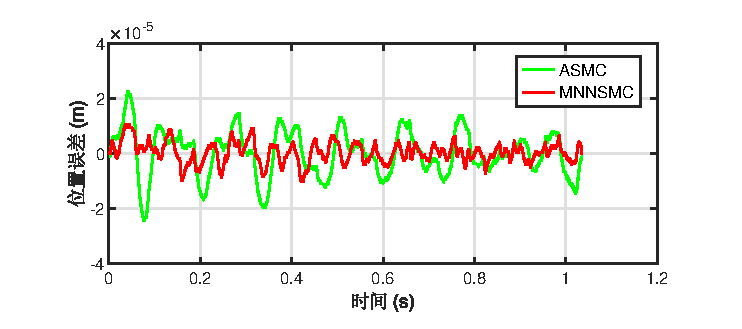
\includegraphics[width=12cm]{figures/S轨迹100有负载.eps}
	\caption{最大速度为100$\,\text{mm$/$s}$的三阶S轨迹有负载情况下位置跟踪误差}
	\label{S轨迹100有负载}
\end{figure}
\begin{figure}[H]
	\centering
	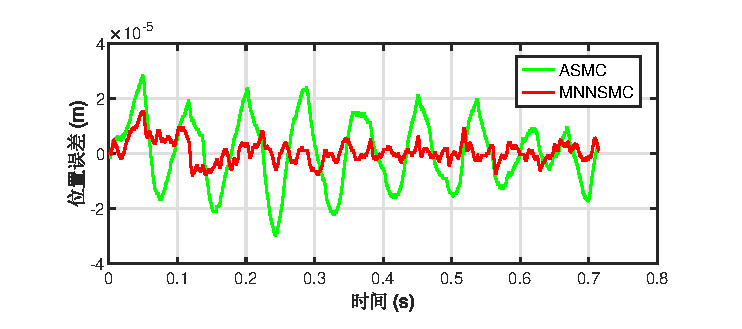
\includegraphics[width=12cm]{figures/S轨迹150有负载.eps}
	\caption{最大速度为150$\,\text{mm$/$s}$的三阶S轨迹有负载情况下位置跟踪误差}
	\label{S轨迹150有负载}
\end{figure}
\begin{figure}[H]
	\centering
	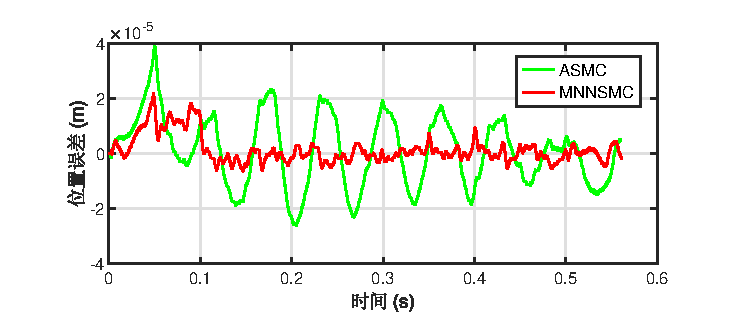
\includegraphics[width=12cm]{figures/S轨迹200有负载.eps}
	\caption{最大速度为200$\,\text{mm$/$s}$的三阶S轨迹有负载情况下位置跟踪误差}
	\label{S轨迹200有负载}
\end{figure}
\end{comment}

\begin{table}[H]
	\caption{实验B中不同参考轨迹位置跟踪性能.}
	\label{实验B}
	\centering
	\setlength{\tabcolsep}{3mm} 
	\begin{tabular}{ccccc}
		\toprule[1.5pt]
		& \text{参考轨迹} & RMSE ($\text{$\upmu$m}$) & MAE ($\text{$\upmu$m}$) & $\text{MAD}$($\text{$\upmu$m}$)   \\ 
		\midrule
		\multirow{5}{*}{ASMC}     
		& 0.5Hz           & 4.13      & 14.2 &3.00   \\ 
		& 1Hz             & 9.06      & 23.2 &6.89   \\ 
		%& C             & 9.57      & 41.4 &0  &0    \\
		& 100\,$\text{mm/s }$            & 7.53      & 19.5 &6.12   \\  
		& 150\,$\text{mm/s }$             & 13.2      & 29.6 &11.5    \\ 
		& 200\,$\text{mm/s }$             & 12.3      & 26.0 &10.5     \\
		\midrule
		\multirow{5}{*}{MNNSMC} 
		& 0.5Hz           & 2.44      & 13.8 &1.77    \\ 
		& 1Hz             & 3.86      & 27.4 &2.31    \\ 
		& 100\,$\text{mm/s }$            & 3.39      & 10.2 &2.70  \\  
		& 150\,$\text{mm/s }$             & 2.82      & 9.20 &2.16     \\ 
		& 200\,$\text{mm/s }$             & 2.41      & 9.40 &1.90     \\
		\bottomrule[1.5pt]
	\end{tabular}
\end{table}

分析表格中的结果,与实验A对比,容易发现,实验B中的各项性能指标与实验A中的各项性能指标仍然保持在同一水平,这充分说明了两种基于神经网络的控制方法对于均能够很好地应对系统模型参数摄动问题,但MNNSMC方法的位置跟踪性能仍然优于ASMC。

对实验A和实验B中不同最大速度的三阶轨迹位置跟踪误差进行了MA和MSD分析,结果如图\ref{不同速度情况下位置跟踪误差MA、MSD曲线}所示。可以清楚地看到,当运行速度提高时,ASMC方法的MA和MSD均有不同程度的增大,而MNNSMC方法的MA和MSD都是稳定地维持在较低水平,这充分说明了MNNSMC方法的位置跟踪性能优于ASMC方法,平均位置误差和定位精度都有很大的提升。

从具体的数值角度来分析,在最大速度为100\,$\text{mm/s}$且无负载情况时,ASMC方法匀速段跟踪误差的MA最大为5.83\,$\text{$\upmu$m}$,MSD最大为11.9\,$\text{$\upmu$m}$,而所提的MNNSMC方法匀速段跟踪误差的MA最大为2.69\,$\text{$\upmu$m}$,MSD最大为4.95\,$\text{$\upmu$m}$,与ASMC方法相比,MNNSMC方法的位置跟踪性能得到了极大的提升。在有负载的情况下,MA和MSD的值也几乎保持一致,MNNSMC方法的MA和MSD分别为2.71\,$\text{$\upmu$m}$和5.07\,$\text{$\upmu$m}$,这一结果从位置跟踪误差的整体性能层面也验证了所提IRLSISMC方法能够有效地提高系统位置跟踪精度,并对系统模型参数摄动有一定的鲁棒性。


\begin{figure}[!t]
	\centering
	\subfloat[100$\,\text{mm/s}$三阶S轨迹无负载]{\label{100mm无负载}%%
		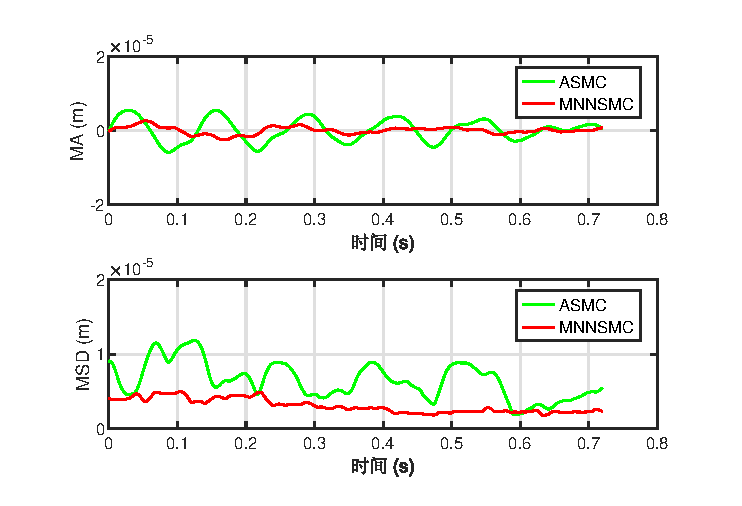
\includegraphics[width=7.5cm]{figures/100mm无负载.eps}} 	
	\subfloat[100$\,\text{mm/s}$三阶S轨迹有负载]{\label{100mm有负载}%%
		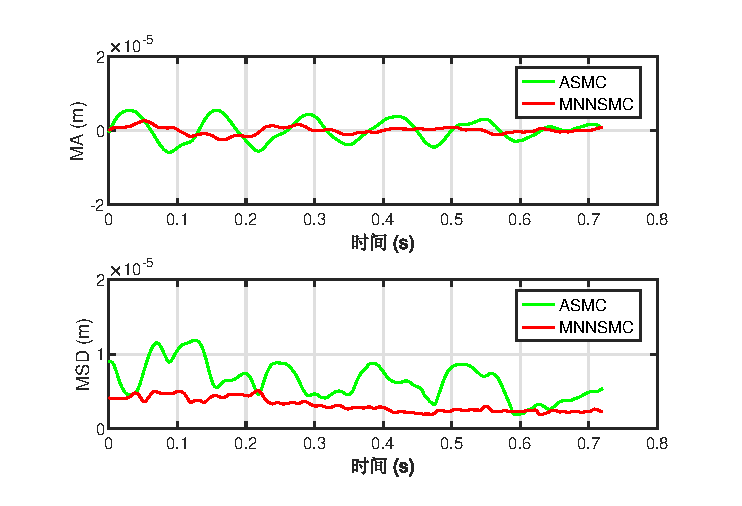
\includegraphics[width=7.5cm]{figures/100mm有负载.eps}} \\
	\subfloat[150$\,\text{mm/s}$三阶S轨迹无负载]{\label{150mm无负载}%%
		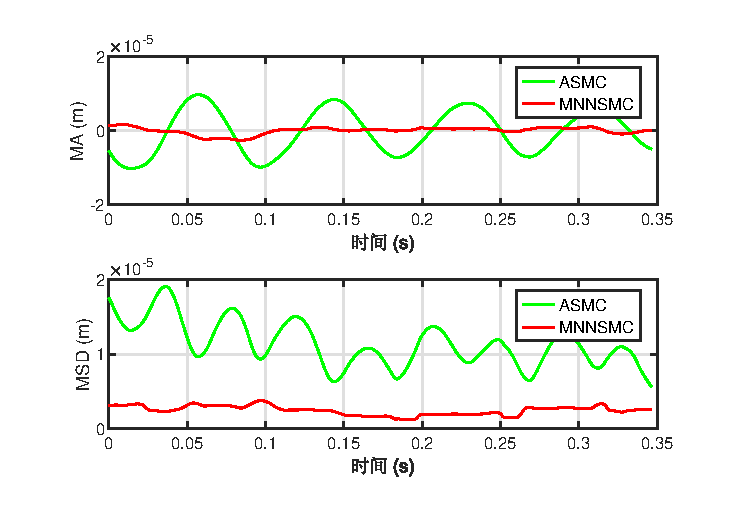
\includegraphics[width=7.5cm]{figures/150mm无负载.eps}} 	
	\subfloat[150$\,\text{mm/s}$三阶S轨迹有负载]{\label{150mm有负载}%%
		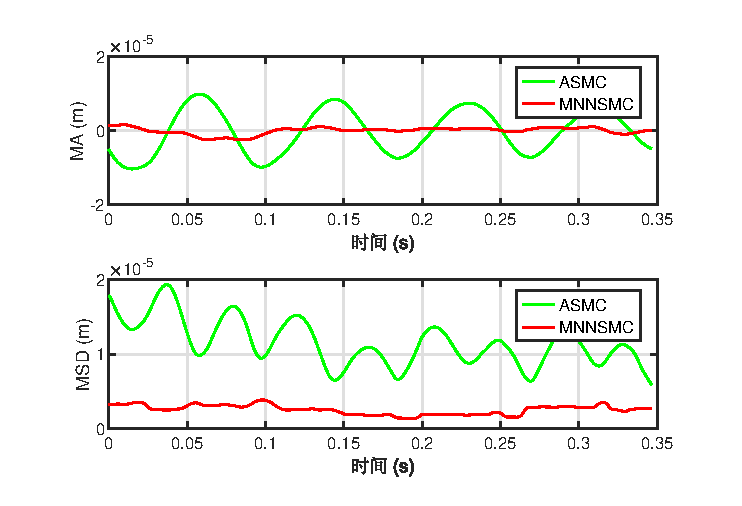
\includegraphics[width=7.5cm]{figures/150mm有负载.eps}} \\
	\subfloat[200$\,\text{mm/s}$三阶S轨迹无负载]{\label{200mm无负载}%%
		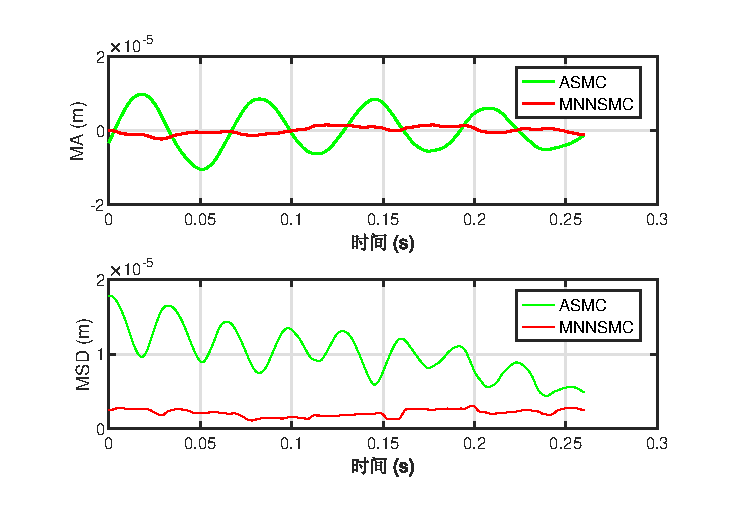
\includegraphics[width=7.5cm]{figures/200mm无负载.eps}} 	
	\subfloat[200$\,\text{mm/s}$三阶S轨迹有负载]{\label{200mm有负载}%%
		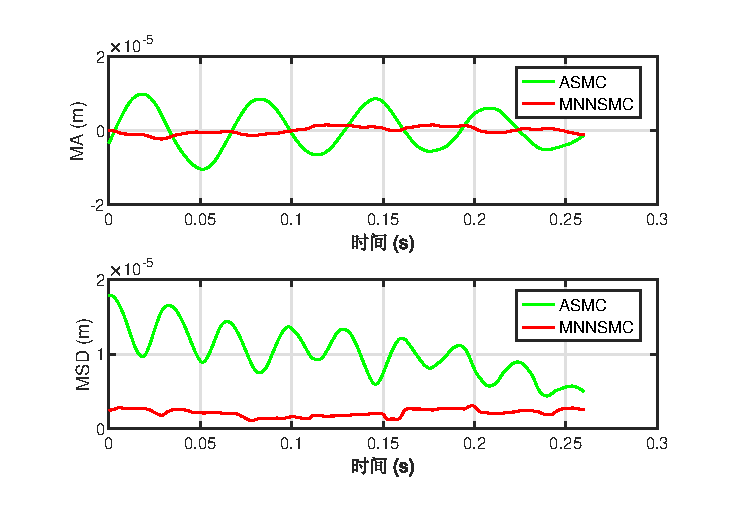
\includegraphics[width=7.5cm]{figures/200mm有负载.eps}} \\
	\caption{不同速度情况下位置跟踪误差MA、MSD曲线}
	\label{不同速度情况下位置跟踪误差MA、MSD曲线}
\end{figure}


在最大速度为200\,$\text{mm/s}$且无负载情况时,ASMC方法匀速段跟踪误差的MA最大为10.4\,$\text{$\upmu$m}$,MSD最大为17.9\,$\text{$\upmu$m}$,而所提的MNNSMC方法匀速段跟踪误差的MA最大为2.23\,$\text{$\upmu$m}$,MSD最大为3.05\,$\text{$\upmu$m}$,说明本文所提的MNNSMC方法较传统ASMC方法有着更好的位置跟踪性能,主要表现在位置跟踪精度高、误差波动范围小以及收敛速度快。纵向对比不同速度情况下匀速段跟踪误差的MA和MSD的变化,可以发现系统运行速度从100\,$\text{mm/s}$到200\,$\text{mm/s}$时,ASMC方法的MA和MSD呈现增长的趋势,但是本文提出的MNNSMC反而有减小的趋势,这主要也是因为动态边界层与速度相关,同时结合多核神经网络的扰动补偿作用,能较好地适应高速高精度的要求。

\begin{comment}
\begin{figure}[H]
	\centering
	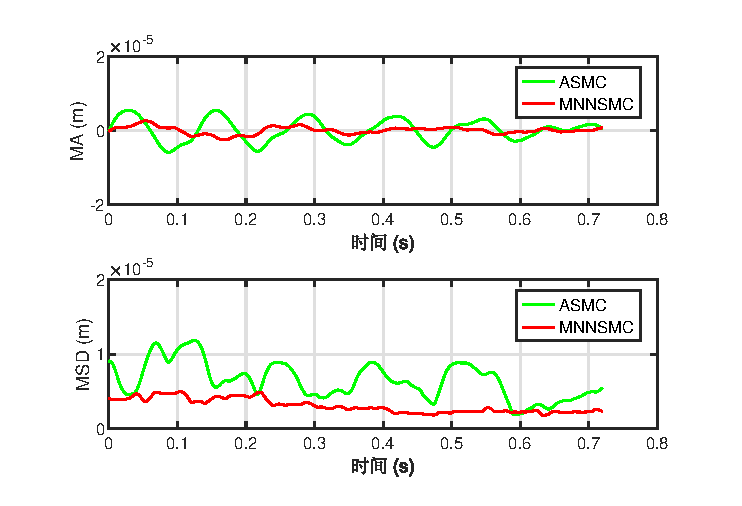
\includegraphics[width=12cm]{figures/100mm无负载.eps}
	\caption{100$\,\text{mm/s}$三阶S轨迹无负载情况下位置跟踪误差MA、MSD曲线}
	\label{100mm无负载}
\end{figure}
\begin{figure}[H]
	\centering
	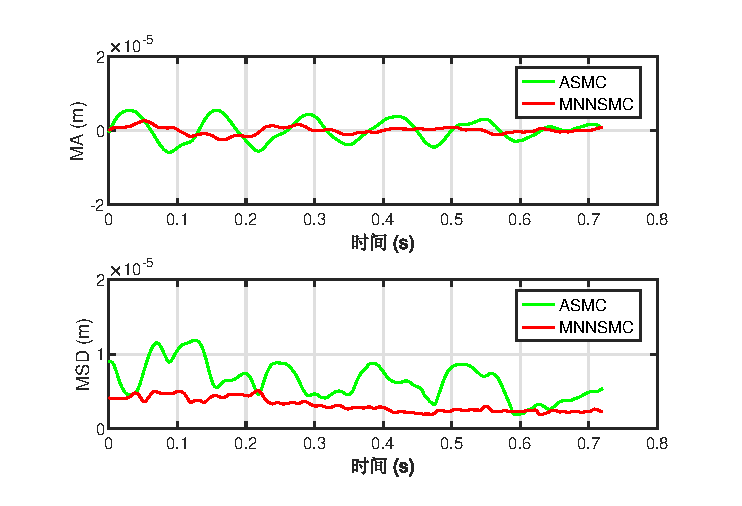
\includegraphics[width=12cm]{figures/100mm有负载.eps}
	\caption{100$\,\text{mm/s}$三阶S轨迹有负载情况下位置跟踪误差MA、MSD曲线}
	\label{100mm有负载}
\end{figure}
\begin{figure}[H]
	\centering
	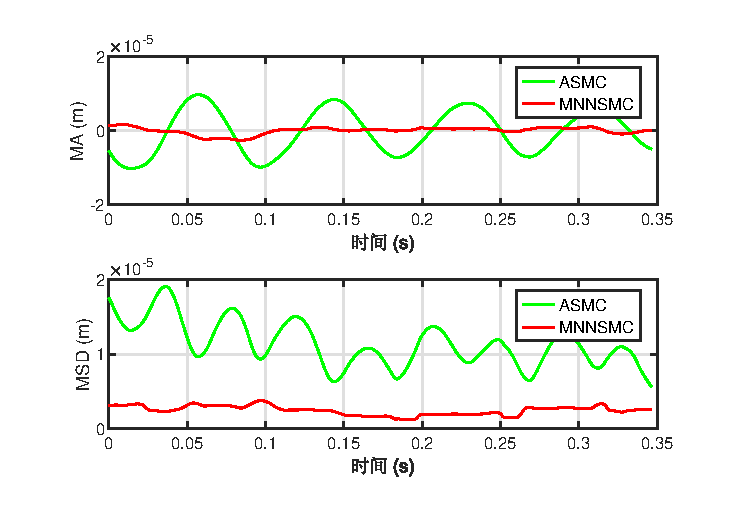
\includegraphics[width=12cm]{figures/150mm无负载.eps}
	\caption{150$\,\text{mm/s}$三阶S轨迹无负载情况下位置跟踪误差MA、MSD曲线}
	\label{150mm无负载}
\end{figure}
\begin{figure}[H]
	\centering
	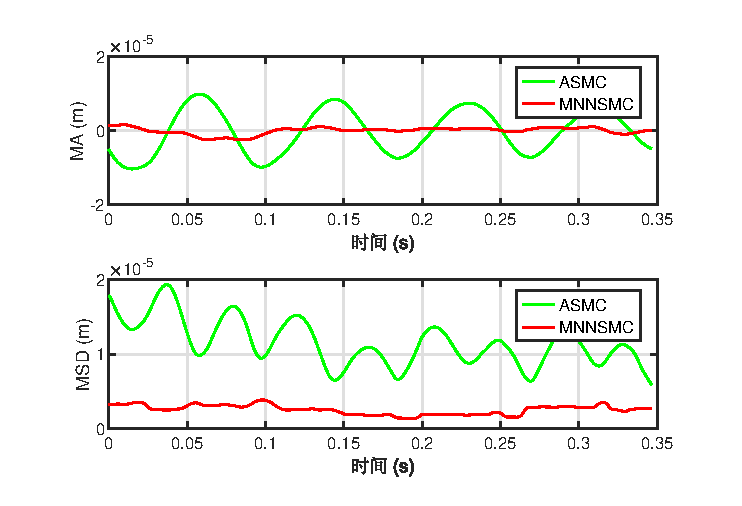
\includegraphics[width=12cm]{figures/150mm有负载.eps}
	\caption{150$\,\text{mm/s}$三阶S轨迹有负载情况下位置跟踪误差MA、MSD曲线}
	\label{150mm有负载}
\end{figure}
\begin{figure}[H]
	\centering
	\includegraphics[width=12cm]{figures/200mm无负载.eps}
	\caption{200$\,\text{mm/s}$三阶S轨迹无负载情况下位置跟踪误差MA、MSD曲线}
	\label{200mm无负载}
\end{figure}
\begin{figure}[H]
	\centering
	\includegraphics[width=12cm]{figures/200mm有负载.eps}
	\caption{200$\,\text{mm/s}$三阶S轨迹有负载情况下位置跟踪误差MA、MSD曲线}
	\label{200mm有负载}
\end{figure}
\end{comment}
(3) 实验C

实验C是在正弦参考轨迹输入情况下,在5\,s时刻加入0.5\,V阶跃扰动并在6\,s时刻移除,用来测试传统ASMC方法与本文提出的MNNSMC方法对系统外界扰动的抑制能力和系统的鲁棒性,其位置跟踪误差如图\ref{不同频率正弦参考轨迹有阶跃扰动情况下位置跟踪误差}所示,可以看到,当系统受到阶跃扰动影响时,所提MNNSMC方法的位置跟踪误差明显低于ASMC方法,具体的各项性能指标如表\ref{实验C}所示。
\begin{figure}[H]\centering
	\subfloat[0.5$\,\text{Hz}$]{\includegraphics[width=12cm]{figures/正弦05Hz有扰动.eps}\label{正弦05Hz有扰动} }\\
	\subfloat[1$\,\text{Hz}$]{\includegraphics[width=12cm]{figures/正弦1Hz有扰动.eps}\label{正弦1Hz有扰动} }
	\caption{不同频率正弦参考轨迹有阶跃扰动情况下位置跟踪误差}\label{不同频率正弦参考轨迹有阶跃扰动情况下位置跟踪误差}
\end{figure}

\begin{comment}
\begin{figure}[H]
	\centering
	\includegraphics[width=12cm]{figures/正弦05Hz有扰动.eps}
	\caption{0.5$\,\text{Hz}$正弦参考轨迹有阶跃扰动情况下位置跟踪误差}
	\label{正弦05Hz有扰动}
\end{figure}
\begin{figure}[H]
	\centering
	\includegraphics[width=12cm]{figures/正弦1Hz有扰动.eps}
	\caption{1$\,\text{Hz}$正弦参考轨迹有阶跃扰动情况下位置跟踪误差}
	\label{正弦1Hz有扰动}
\end{figure}
\end{comment}

\begin{table}[H]
	\caption{实验C中不同参考轨迹位置跟踪性能.}
	\label{实验C}
	\centering
	\setlength{\tabcolsep}{3mm} 
	\begin{tabular}{ccccc}
		\toprule[1.5pt]
		& \text{参考轨迹} & RMSE ($\text{$\upmu$m}$) & MAE ($\text{$\upmu$m}$) & $\text{MAD}$($\text{$\upmu$m}$)   \\ 
		\midrule
		\multirow{2}{*}{ASMC}     
		& 0.5\,Hz           & 5.12      & 50.4 &3.22  \\ 
		& 1\,Hz             & 9.57      & 41.4 &7.07  \\ 
		%& C             & 9.57      & 41.4 &0  &0  \\
		\midrule
		\multirow{2}{*}{MNNSMC} 
		& 0.5\,Hz           & 3.36      & 25.9 &2.45  \\ 
		& 1\,Hz             & 5.03      & 27.6 &3.36  \\ 
		\bottomrule[1.5pt]
	\end{tabular}
\end{table}

分析表格中的结果,容易发现,ASMC方法在低速情况下受到阶跃扰动的影响,使得MAE为$50.4\,\upmu$$\text{m}$,这一结果要比高速情况下受到阶跃扰动的影响更大,这是由于ASMC方法在低速情况下虽然也能够保证系统的位置跟踪精度,比如RMSE和MAD也都维持在较低水平,但是对于阶跃扰动的补偿需要一定的时间。而高速情况下,由于系统本身扰动影响较大,ASMC的补偿项稳定情况下已经发挥较大作用,因此在同样幅值的阶跃扰动影响下,MAE的值影响较低速情况略微缓和。而MNNSMC方法在低速和高速情况下的位置跟踪性能指标均维持相对稳定的水平,这进一步表明MNNSMC方法拥有较好的扰动抑制能力。

(4)为了验证动态边界层的效果,在不同边界层情况下对提出的MNNSMC方法进行了实验验证,为了方便,这里仅在最大速度为$200\,\text{mm/s}$的三阶轨迹输入时进行测试,得到的位置跟踪误差曲线如图\ref{不同边界层}所示。显然,动态边界层能够进一步提高系统的位置跟踪精度。
\begin{figure}[H]
	\centering
	\includegraphics[width=12cm]{figures/不同边界层.eps}
	\caption{不同边界层情况下$200\,\text{mm/s}$三阶轨迹的位置跟踪误差曲线}
	\label{不同边界层}
\end{figure}
\begin{comment}
实验B中,在实验A的基础上添加了$0.437\,\text{kg}$负载,测试传统RBF神经网络滑模控制方法(ASMC)与提出的多核神经网络动态边界层滑模控制方法(MNNSMC)对系统参数变化的鲁棒性,其位置跟踪误差如图\ref{正弦05有负载}所示。
\begin{figure}[H]
	\centering
	\includegraphics[width=12cm]{figures/正弦05Hz有负载.eps}
	\caption{0.5$\,\text{Hz}$正弦参考轨迹有负载情况下位置跟踪误差}
	\label{正弦05有负载}
\end{figure}
实验C中,添加了$0.5\,\text{V}$阶跃扰动,测试传统RBF神经网络滑模控制方法(ASMC)与提出的多核神经网络动态边界层滑模控制方法(MNNSMC)对系统外界扰动的鲁棒性,其位置跟踪误差如图\ref{正弦05Hz有扰动}所示。
\begin{figure}[H]
	\centering
	\includegraphics[width=12cm]{figures/正弦05Hz有扰动.eps}
	\caption{0.5$\,\text{Hz}$正弦参考轨迹有阶跃扰动情况下位置跟踪误差}
	\label{正弦05Hz有扰动}
\end{figure}


(2) 1$\,\text{Hz}$正弦参考轨迹

实验A中,系统名义模型采用事先辨识好的等效质量$M=\text{0.12$\,$Vs$^{2}$/m}$,测试传统RBF神经网络滑模控制方法(ASMC)与提出的多核神经网络动态边界层滑模控制(MNNSMC)在名义模型下的位置跟踪性能,其位置跟踪性能如图\ref{正弦1Hz无负载}所示。
\begin{figure}[H]
	\centering
	\includegraphics[width=12cm]{figures/正弦1Hz无负载.eps}
	\caption{1$\,\text{Hz}$正弦参考轨迹名义模型情况下位置跟踪误差}
	\label{正弦1Hz无负载}
\end{figure}
实验B中,在实验A的基础上添加了$0.437\,\text{kg}$负载,测试传统RBF神经网络滑模控制方法(ASMC)与提出的多核神经网络动态边界层滑模控制方法(MNNSMC)对系统参数变化的鲁棒性,其位置跟踪误差如图\ref{正弦1Hz有负载}所示。
\begin{figure}[H]
	\centering
	\includegraphics[width=12cm]{figures/正弦1Hz有负载.eps}
	\caption{1$\,\text{Hz}$正弦参考轨迹有负载情况下位置跟踪误差}
	\label{正弦1Hz有负载}
\end{figure}
实验C中,添加了$0.5\,\text{V}$阶跃扰动,测试传统RBF神经网络滑模控制方法(ASMC)与提出的多核神经网络动态边界层滑模控制方法(MNNSMC)对系统外界扰动的鲁棒性,其位置跟踪误差如图\ref{正弦1Hz有扰动}所示。
\begin{figure}[H]
	\centering
	\includegraphics[width=12cm]{figures/正弦1Hz有扰动.eps}
	\caption{1$\,\text{Hz}$正弦参考轨迹有阶跃扰动情况下位置跟踪误差}
	\label{正弦1Hz有扰动}
\end{figure}

(3) 最大速度为100$\,\text{mm$/$s}$的三阶S轨迹

实验A中,系统名义模型采用事先辨识好的等效质量$M=\text{0.12$\,$Vs$^{2}$/m}$,测试传统RBF神经网络滑模控制方法(ASMC)与提出的多核神经网络动态边界层滑模控制(MNNSMC)在名义模型下的位置跟踪性能,其位置跟踪性能如图\ref{S轨迹100无负载}所示。
\begin{figure}[H]
	\centering
	\includegraphics[width=12cm]{figures/S轨迹100无负载.eps}
	\caption{最大速度为100$\,\text{mm$/$s}$的三阶S轨迹名义模型情况下位置跟踪误差}
	\label{S轨迹100无负载}
\end{figure}

实验B中,在实验A的基础上添加了$0.437\,\text{kg}$负载,测试传统RBF神经网络滑模控制方法(ASMC)与提出的多核神经网络动态边界层滑模控制方法(MNNSMC)对系统参数变化的鲁棒性,其位置跟踪误差如图\ref{S轨迹100有负载}所示。
\begin{figure}[H]
	\centering
	\includegraphics[width=12cm]{figures/S轨迹100有负载.eps}
	\caption{最大速度为100$\,\text{mm$/$s}$的三阶S轨迹有负载情况下位置跟踪误差}
	\label{S轨迹100有负载}
\end{figure}

(4) 最大速度为150$\,\text{mm$/$s}$的三阶S轨迹

实验A中,系统名义模型采用事先辨识好的等效质量$M=\text{0.12$\,$Vs$^{2}$/m}$,测试传统RBF神经网络滑模控制方法(ASMC)与提出的多核神经网络动态边界层滑模控制(MNNSMC)在名义模型下的位置跟踪性能,其位置跟踪性能如图\ref{S轨迹150无负载}所示。
\begin{figure}[H]
	\centering
	\includegraphics[width=12cm]{figures/S轨迹150无负载.eps}
	\caption{最大速度为150$\,\text{mm$/$s}$的三阶S轨迹名义模型情况下位置跟踪误差}
	\label{S轨迹150无负载}
\end{figure}

实验B中,在实验A的基础上添加了$0.437\,\text{kg}$负载,测试传统RBF神经网络滑模控制方法(ASMC)与提出的多核神经网络动态边界层滑模控制方法(MNNSMC)对系统参数变化的鲁棒性,其位置跟踪误差如图\ref{S轨迹150有负载}所示。
\begin{figure}[H]
	\centering
	\includegraphics[width=12cm]{figures/S轨迹150有负载.eps}
	\caption{最大速度为150$\,\text{mm$/$s}$的三阶S轨迹有负载情况下位置跟踪误差}
	\label{S轨迹150有负载}
\end{figure}

(5) 最大速度为200$\,\text{mm$/$s}$的三阶S轨迹

实验A中,系统名义模型采用事先辨识好的等效质量$M=\text{0.12$\,$Vs$^{2}$/m}$,测试传统RBF神经网络滑模控制方法(ASMC)与提出的多核神经网络动态边界层滑模控制(MNNSMC)在名义模型下的位置跟踪性能,其位置跟踪性能如图\ref{S轨迹200无负载}所示。
\begin{figure}[H]
	\centering
	\includegraphics[width=12cm]{figures/S轨迹200无负载.eps}
	\caption{最大速度为200$\,\text{mm$/$s}$的三阶S轨迹名义模型情况下位置跟踪误差}
	\label{S轨迹200无负载}
\end{figure}

实验B中,在实验A的基础上添加了$0.437\,\text{kg}$负载,测试传统RBF神经网络滑模控制方法(ASMC)与提出的多核神经网络动态边界层滑模控制方法(MNNSMC)对系统参数变化的鲁棒性,其位置跟踪误差如图\ref{S轨迹200有负载}所示。
\begin{figure}[H]
	\centering
	\includegraphics[width=12cm]{figures/S轨迹200有负载.eps}
	\caption{最大速度为200$\,\text{mm$/$s}$的三阶S轨迹有负载情况下位置跟踪误差}
	\label{S轨迹200有负载}
\end{figure}
\end{comment}
\section{本章小结}
本章对所提控制方法进行了实验验证,实验对象为精密直线运动平台,通过4种位置跟踪误差性能评价指标对实验结果进行了分析,充分表明了所提方法在精密直线运动平台上良好的控制性能。通过输入不同的三阶轨迹对提出的IRLSISMC方法进行了实验验证,实验结果表明了引入定位力主要成分的改进型RLS能够有效地提高三阶轨迹匀速段的跟踪性能,与传统的TRLSISMC方法相比,其RMSE能够维持在4\,$\upmu$m附近,MAE能够维持在11\,$\upmu$m附近,200\,$\upmu$m三阶轨迹跟踪实验中,MA、MSD也能够保持较好的水平。通过输入不同频率的正弦参考轨迹和不同速度的三阶轨迹对提出的MNNSMC方法进行了实验验证,并与传统ASMC方法进行比较,实验结果表明,本文提出的MNNSMC方法能够更有效地提高系统的位置跟踪性能和抗干扰能力。
%\newpage
%\mbox{}
%\newpage